\documentclass[11pt,a4paper]{article}

\usepackage[margin=2.4cm]{geometry}
\usepackage[utf8]{inputenc}
\usepackage[expansion=false]{microtype}
\usepackage{amsmath,amssymb,amsthm}
\usepackage{booktabs,array,enumitem,xcolor,float}
\usepackage{graphicx}
\usepackage{tikz}
\usetikzlibrary{arrows.meta,calc,decorations.markings,angles,quotes,positioning,patterns}
\usepackage{pgfplots}
\pgfplotsset{compat=1.16}
\usepackage[most]{tcolorbox}
\usepackage[colorlinks=true,linkcolor=blue!50!black,urlcolor=blue!50!black]{hyperref}

\setlength{\parskip}{4pt}
\setlength{\parindent}{0pt}

% ---------- macros ----------
\newcommand{\R}{\mathbb{R}}
\newcommand{\W}{\mathcal{W}}
\newcommand{\C}{\mathcal{C}}
\newcommand{\SO}{\mathrm{SO}}
\newcommand{\SE}{\mathrm{SE}}
\newcommand{\Sph}{\mathbb{S}}
\newcommand{\norm}[1]{\lVert #1\rVert}
\newcommand{\pts}[1]{\emph{(notes p.~#1)}}

% TikZ helpers (AMR02)
\newcommand{\photobox}[2]{\fbox{\parbox[c][#1][c]{0.29\linewidth}{\centering
  \color{red!70!black}\textbf{[Blank --- insert image]}\par\scriptsize\color{black}#2}}}
\newcommand{\com}[1]{\begin{scope}[shift={(#1)}]\draw[fill=white,thick] (0,0) circle (0.13);
  \fill (0,0) -- (0.13,0) arc (0:90:0.13) -- cycle;
  \fill (0,0) -- (-0.13,0) arc (180:270:0.13) -- cycle;\end{scope}}
\newcommand{\zmpmark}[1]{\begin{scope}[shift={(#1)}]\draw[red!70!black,very thick]
  (-0.12,-0.12)--(0.12,0.12) (-0.12,0.12)--(0.12,-0.12);\end{scope}}
\newcommand{\fixedwheel}[2]{\begin{scope}[shift={(#1)},rotate=#2]
  \draw[fill=gray!30] (-0.3,-0.07) rectangle (0.3,0.07);\end{scope}}
\newcommand{\orientwheel}[2]{\begin{scope}[shift={(#1)},rotate=#2]
  \draw[pattern=north east lines] (-0.3,-0.07) rectangle (0.3,0.07);
  \fill (0,0) circle (1pt);\end{scope}}
\newcommand{\casterwheel}[2]{\begin{scope}[shift={(#1)},rotate=#2]
  \draw (0,0)--(-0.4,0); \draw[fill=white] (-0.6,-0.06) rectangle (-0.2,0.06);
  \fill (0,0) circle (1.5pt);\end{scope}}
\newcommand{\ghostwheel}[2]{\begin{scope}[shift={(#1)},rotate=#2]
  \draw[dashed,gray] (-0.3,-0.07) rectangle (0.3,0.07);\end{scope}}

% ---------- theorem environments ----------
\theoremstyle{definition}
\newtheorem{definition}{Definition}[section]
\newtheorem{example}[definition]{Example}
\newtheorem{algorithm}[definition]{Algorithm}
\theoremstyle{plain}
\newtheorem{lemma}[definition]{Lemma}
\newtheorem{theorem}[definition]{Theorem}
\newtheorem{proposition}[definition]{Proposition}
\newtheorem{corollary}[definition]{Corollary}

\tcbset{
  thmbox/.style={enhanced,breakable,colback=gray!4,colframe=gray!60!black,
    boxrule=0.6pt,arc=2pt,left=6pt,right=6pt,top=4pt,bottom=4pt}
}
\tcolorboxenvironment{definition}{thmbox}
\tcolorboxenvironment{example}{thmbox}
\tcolorboxenvironment{algorithm}{thmbox}
\tcolorboxenvironment{lemma}{thmbox}
\tcolorboxenvironment{proposition}{thmbox}
\tcolorboxenvironment{theorem}{thmbox}
\tcolorboxenvironment{corollary}{thmbox}

\newtcolorbox{intuition}{enhanced,breakable,colback=blue!5,colframe=blue!55!black,
  fonttitle=\bfseries,title={Intuition},boxrule=0.6pt,arc=2pt,
  left=6pt,right=6pt,top=3pt,bottom=3pt}

\graphicspath{{/home/vittorio/Desktop/AIRO/AMR/tex/AMR01/}{/home/vittorio/Desktop/AIRO/AMR/tex/AMR02/}{/home/vittorio/Desktop/AIRO/AMR/tex/AMR03/}}

\title{\textbf{Autonomous and Mobile Robotics}\\[6pt]\large Comprehensive Lecture Notes}
\author{Vittorio Cava}
\date{A.Y.~2026/27}

\begin{document}
\maketitle
\tableofcontents
\newpage

% ======================================================================
% Lecture 1
% ======================================================================
\part{Lecture 1}

% =====================================================================
\section{Configuration Space and Workspace}\pts{1--2}
% =====================================================================

\subsection{The idea}

The central idea is to \emph{define a suitable space in which the robot is a single point}. Once the robot is a point, two core tasks become much simpler to formulate:
\begin{itemize}[nosep]
  \item \textbf{planning} (find a path for the point from a start to a goal),
  \item \textbf{control} (make the point follow that path).
\end{itemize}
(Fun fact from the notes: the C-space concept was born to do \emph{collision avoidance}.)

\begin{intuition}
Think of a huge, awkwardly shaped sofa that has to be moved through a door. Reasoning about every corner of the sofa at the same time is painful. If instead we find a space where the whole sofa is \emph{one dot}, and the ``forbidden'' places for the dot are exactly the sofa positions that hit a wall, then moving the sofa becomes moving a dot around obstacles.
\end{intuition}

\subsection{Robots and workspaces}

\begin{definition}[Robot and workspace]
A \emph{robot} is a collection of $n_b$ rigid bodies (we assume rigid robots) moving in a \emph{workspace} $\W=\R^2$ or $\W=\R^3$, the physical space in which the robot moves.
\begin{itemize}[nosep]
  \item If $\W=\R^2$ the robot is \emph{planar}; if $\W=\R^3$ it is \emph{spatial}.
  \item If $n_b=1$ the robot is \emph{single-body}; if $n_b>1$ it is \emph{multi-body}.
\end{itemize}
\end{definition}

\begin{example}
A car can be modelled as a single body, whereas a car with a trailer is a multi-body system ($n_b=2$).
\end{example}

\subsection{Configuration and generalized coordinates}

\begin{definition}[Posture and configuration]
The \emph{posture} of a robot is the position of all its points in $\W$. A \emph{configuration} is a \emph{minimal} set of parameters that defines the posture of the robot in $\W$. The corresponding vector
\[
  q=\begin{pmatrix} q_1\\ \vdots\\ q_n\end{pmatrix}
\]
is called a \emph{configuration vector}, and each $q_i$ is a \emph{generalized coordinate}.
\end{definition}

The generalized coordinates are of two kinds:
\begin{itemize}[nosep]
  \item \textbf{Cartesian coordinates}: identify the position of representative points of the robot; they take values in $\R^2$ or $\R^3$.
  \item \textbf{Angular coordinates}: identify the orientation of the bodies of the robot; they take values in $\SO(2)$ (planar: one parameter) or $\SO(3)$ (spatial: three parameters).
\end{itemize}


\begin{figure}[ht]
\centering
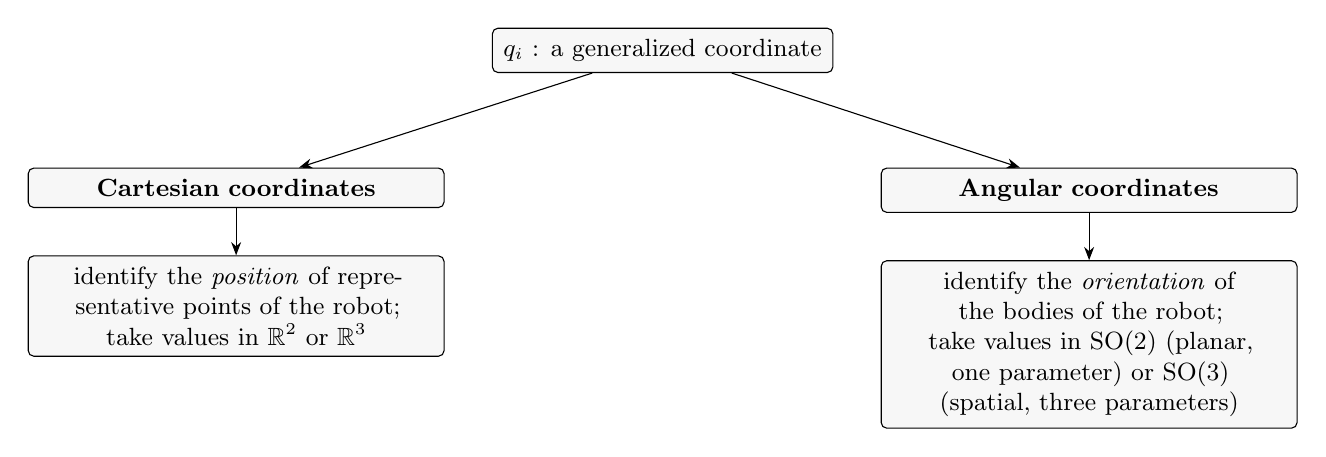
\begin{tikzpicture}[>=Stealth,node distance=8mm,
  box/.style={draw,rounded corners=2pt,fill=gray!6,align=center,inner sep=4pt,font=\small}]
  \node[box] (q) {$q_i$ : a generalized coordinate};
  \node[box,below left=12mm and 6mm of q,text width=5cm] (c) {\textbf{Cartesian coordinates}};
  \node[box,below right=12mm and 6mm of q,text width=5cm] (a) {\textbf{Angular coordinates}};
  \node[box,below=6mm of c,text width=5cm] (c2) {identify the \emph{position} of representative points of the robot;\\ take values in $\R^2$ or $\R^3$};
  \node[box,below=6mm of a,text width=5cm] (a2) {identify the \emph{orientation} of the bodies of the robot;\\ take values in $\SO(2)$ (planar, one parameter) or $\SO(3)$ (spatial, three parameters)};
  \draw[->] (q) -- (c); \draw[->] (q) -- (a);
  \draw[->] (c) -- (c2); \draw[->] (a) -- (a2);
\end{tikzpicture}
\caption{The two kinds of generalized coordinates.}
\end{figure}

\begin{intuition}
``Minimal'' is the key word. The posture is the full, redundant description (every point of every body); the configuration is the shortest list of numbers from which the posture can be reconstructed. A rigid rectangle in the plane has infinitely many points, but three numbers $(x,y,\theta)$ tell you where all of them are.
\end{intuition}

\subsection{Configuration space}

\begin{definition}[Configuration space]
The \emph{configuration space} (C-space) $\C$ of a robot is the set of all possible values of $q$. Its dimension $n=\dim\C$ is the number of degrees of freedom of the robot.
\end{definition}

\begin{intuition}
The C-space is the ``catalogue of all poses the robot can be in''. Each point of $\C$ \emph{is} one pose. A curve in $\C$ is therefore a motion of the robot in the physical space, which is exactly why planning for a robot reduces to planning for a point.
\end{intuition}

% =====================================================================
\section{Examples of Configuration Spaces}\pts{2--3}
% =====================================================================

\begin{example}[Point robot in $\W=\R^3$]
$q=(x,y,z)^\top$, so $\C=\R^3=\W$ and $n=3$.
\end{example}

\begin{example}[Disk robot in $\W=\R^2$]
Since a disk looks the same under any rotation, its orientation is irrelevant: $q=(x,y)^\top$, $\C=\R^2=\W$, $n=2$.
\end{example}

\begin{figure}[ht]
\centering
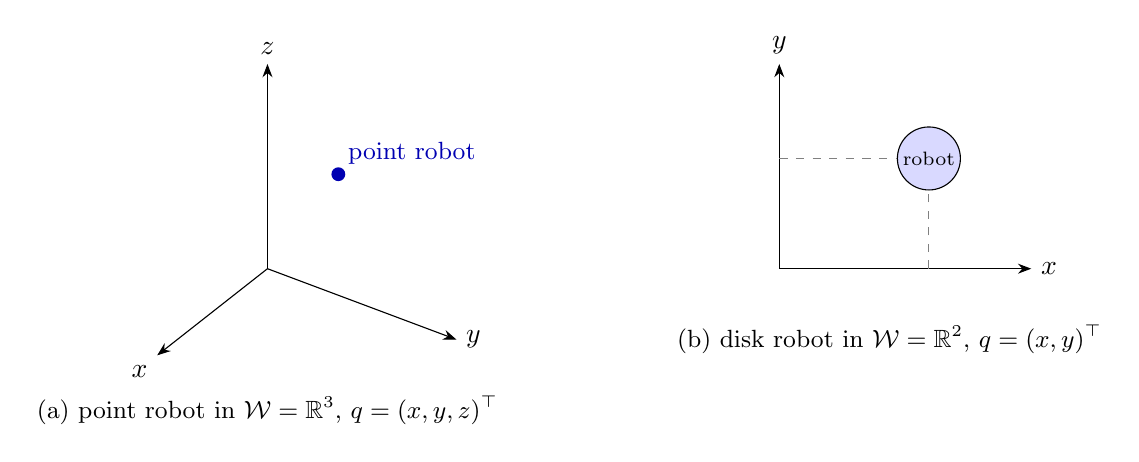
\begin{tikzpicture}[>=Stealth]
  % point robot in R^3
  \begin{scope}
    \draw[->] (0,0) -- (0,2.6) node[above] {$z$};
    \draw[->] (0,0) -- (2.4,-0.9) node[right] {$y$};
    \draw[->] (0,0) -- (-1.4,-1.1) node[below left] {$x$};
    \fill[blue!70!black] (0.9,1.2) circle (2.5pt) node[above right] {\small point robot};
    \node at (0,-1.8) {\small (a) point robot in $\W=\R^3$, $q=(x,y,z)^\top$};
  \end{scope}
  % disk robot in R^2
  \begin{scope}[shift={(6.5,0)}]
    \draw[->] (0,0) -- (3.2,0) node[right] {$x$};
    \draw[->] (0,0) -- (0,2.6) node[above] {$y$};
    \draw[fill=blue!15] (1.9,1.4) circle (0.4);
    \node at (1.9,1.4) {\scriptsize robot};
    \draw[dashed,gray] (0,1.4) -- (1.5,1.4);
    \draw[dashed,gray] (1.9,0) -- (1.9,1.0);
    \node at (1.4,-0.9) {\small (b) disk robot in $\W=\R^2$, $q=(x,y)^\top$};
  \end{scope}
\end{tikzpicture}
\caption{Point robot and disk robot: in both cases $\C=\W$.}
\end{figure}

In both examples $\C$ and $\W$ coincide. A case where they differ:

\begin{example}[Disk with a tick]
We add a small mark (a ``tick'') to the disk, so that its orientation now matters. Then
\[
  q=\begin{pmatrix}x\\y\\\varphi\end{pmatrix},\qquad
  \C=\R^2\times \SO(2),\qquad n=3 ,
\]
where $\times$ is the Cartesian product.
\end{example}

\begin{figure}[ht]
\centering
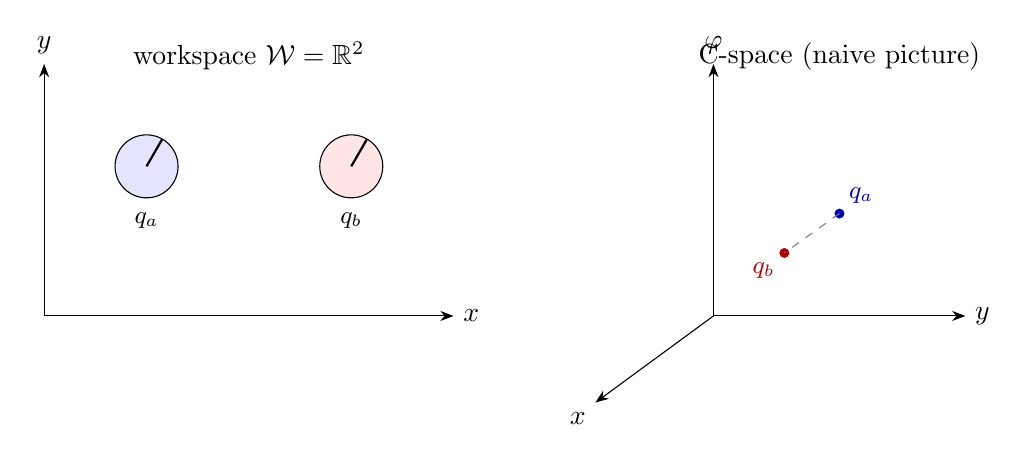
\begin{tikzpicture}[scale=1,>=Stealth]
% ---- workspace ----
\begin{scope}
  \draw[->] (0,0) -- (5.2,0) node[right] {$x$};
  \draw[->] (0,0) -- (0,3.2) node[above] {$y$};
  \node at (2.6,3.3) {workspace $\W=\R^2$};
  % configuration a
  \begin{scope}[shift={(1.3,1.9)}]
    \draw[fill=blue!10] (0,0) circle (0.4);
    \draw[thick] (0,0) -- (60:0.4);
    \node[below=2pt] at (0,-0.4) {\small $q_a$};
  \end{scope}
  % configuration b: same y and phi, different x
  \begin{scope}[shift={(3.9,1.9)}]
    \draw[fill=red!10] (0,0) circle (0.4);
    \draw[thick] (0,0) -- (60:0.4);
    \node[below=2pt] at (0,-0.4) {\small $q_b$};
  \end{scope}
\end{scope}
% ---- configuration space ----
\begin{scope}[shift={(8.5,0)}]
  \draw[->] (0,0) -- (0,3.2) node[above] {$\varphi$};
  \draw[->] (0,0) -- (3.2,0) node[right] {$y$};
  \draw[->] (0,0) -- (-1.5,-1.1) node[below left] {$x$};
  \node at (1.6,3.3) {C-space (naive picture)};
  \coordinate (qa) at (-0.4,-0.3);
  \coordinate (qb) at (-1.1,-0.8);
  \fill[blue!70!black] ($(qa)+(2.0,1.6)$) circle (1.8pt) node[above right] {\small $q_a$};
  \fill[red!70!black]  ($(qb)+(2.0,1.6)$) circle (1.8pt) node[below left] {\small $q_b$};
  \draw[dashed,gray] ($(qa)+(2.0,1.6)$) -- ($(qb)+(2.0,1.6)$);
\end{scope}
\end{tikzpicture}
\caption{The disk with a tick. Configurations $q_a$ and $q_b$ have the same $y$ and $\varphi$ but different $x$. In C-space they differ only along the $x$-axis. (This picture is \emph{naive}: it is not topologically correct, see Section~\ref{sec:topology}.)}
\end{figure}

\noindent Every change in the configuration space is a path, i.e.\ a motion, in the physical space.

\begin{example}[Polygonal robot in $\W=\R^2$]
For instance a car moving on the ground. It can rotate about its centre of mass:
\[
  q=\begin{pmatrix}x\\y\\\theta\end{pmatrix},\quad \C=\R^2\times\SO(2),\quad n=3.
\]
\end{example}

\begin{figure}[ht]
\centering
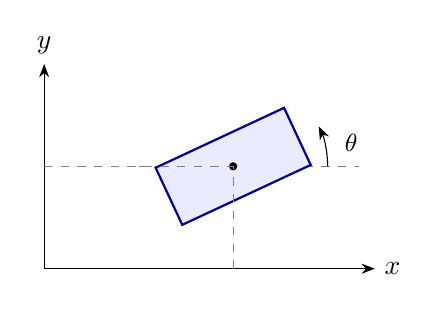
\begin{tikzpicture}[>=Stealth]
  \draw[->] (0,0) -- (4.2,0) node[right] {$x$};
  \draw[->] (0,0) -- (0,2.6) node[above] {$y$};
  \begin{scope}[shift={(2.4,1.3)}]
    \draw[dashed,gray] (-1.2,0) -- (1.6,0);
    \begin{scope}[rotate=25]
      \draw[thick,blue!60!black,fill=blue!8] (-0.9,-0.4) rectangle (0.9,0.4);
    \end{scope}
    \fill (0,0) circle (1.5pt);
    \draw[->] (1.2,0) arc (0:25:1.2);
    \node at (1.5,0.3) {\small $\theta$};
  \end{scope}
  \draw[dashed,gray] (0,1.3) -- (2.4,1.3);
  \draw[dashed,gray] (2.4,0) -- (2.4,1.3);
\end{tikzpicture}
\caption{Polygonal robot in the plane: position of the centre of mass $(x,y)$ and orientation $\theta$.}
\end{figure}

\begin{example}[Polyhedral robot in $\W=\R^3$]
Treat it like the previous case, but add $z$ and two more orientation angles:
\[
  q=(x,y,z,\alpha,\beta,\gamma)^\top,\qquad \C=\R^3\times\SO(3),\qquad n=6.
\]
\end{example}

\begin{definition}[Special Euclidean groups]
The spaces $\R^2\times\SO(2)$ and $\R^3\times\SO(3)$ are called the \emph{special Euclidean groups}, denoted $\SE(2)$ and $\SE(3)$.
\end{definition}

\begin{intuition}
$\SE(n)$ is the set of all rigid motions (a rotation followed by a translation) of $n$-dimensional space. A free rigid body can be moved anywhere and turned any way, so its configuration space is exactly the set of rigid motions: $3$ numbers in the plane ($2$ translations + $1$ rotation), $6$ in space ($3$ translations + $3$ rotations).
\end{intuition}

% =====================================================================
\section{Multi-Body Robots: Manipulators}\pts{4--5}
% =====================================================================

\subsection{Planar manipulator with $n_b$ links}

Consider a planar manipulator with $n_b$ links and $n_b$ (e.g.\ revolute) joints moving in $\W=\R^2$. Each link is a rigid body with 3 degrees of freedom in the plane, so one might expect $3n_b$ generalized coordinates. This is wrong: the links are \emph{connected}, and every joint introduces constraints.

\begin{proposition}[Degrees of freedom of a planar serial arm]
A planar arm of $n_b$ links connected to the ground by $n_b$ revolute joints has
\[
  3n_b-2n_b=n_b
\]
degrees of freedom. Each revolute joint imposes $2$ constraints (the two coordinates of the joint point must coincide on the two bodies it connects).
\end{proposition}

Hence, to describe the configuration we do not need to remember all the constraints: one angle per joint is enough,
\[
  q=\begin{pmatrix}q_1\\q_2\\\vdots\\q_{n_b}\end{pmatrix},\quad n=n_b,\qquad
  \C=\underbrace{\SO(2)\times\dots\times\SO(2)}_{n_b\text{ times}}=\SO(2)^{n_b}.
\]

\begin{figure}[ht]
\centering
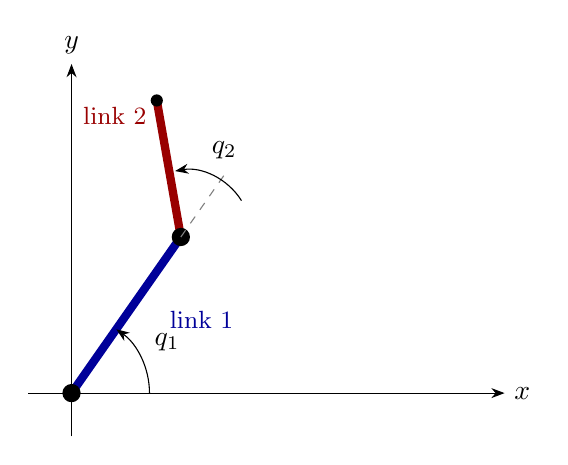
\begin{tikzpicture}[>=Stealth,scale=1.1]
  \draw[->] (-0.5,0) -- (5,0) node[right] {$x$};
  \draw[->] (0,-0.5) -- (0,3.8) node[above] {$y$};
  \coordinate (O) at (0,0);
  \coordinate (J) at (55:2.2);
  \coordinate (E) at ($(J)+(100:1.6)$);
  \draw[line width=3pt,blue!60!black] (O) -- (J);
  \draw[line width=3pt,red!60!black] (J) -- (E);
  \fill (O) circle (3pt);
  \fill (J) circle (3pt);
  \fill (E) circle (2pt);
  \draw[dashed,gray] (J) -- ($(J)+(55:0.9)$);
  \draw[->] (0.9,0) arc (0:55:0.9);
  \node at (28:1.25) {$q_1$};
  \draw[->] ($(J)+(0.7,0.42)$) arc (32:100:0.75) ;
  \node at ($(J)+(0.5,1.0)$) {$q_2$};
  \node[blue!60!black] at (1.5,0.85) {\small link 1};
  \node[red!60!black] at (0.5,3.2) {\small link 2};
\end{tikzpicture}
\caption{A 2R planar arm: one angle per joint is enough to describe the configuration.}
\end{figure}


\begin{figure}[ht]
\centering
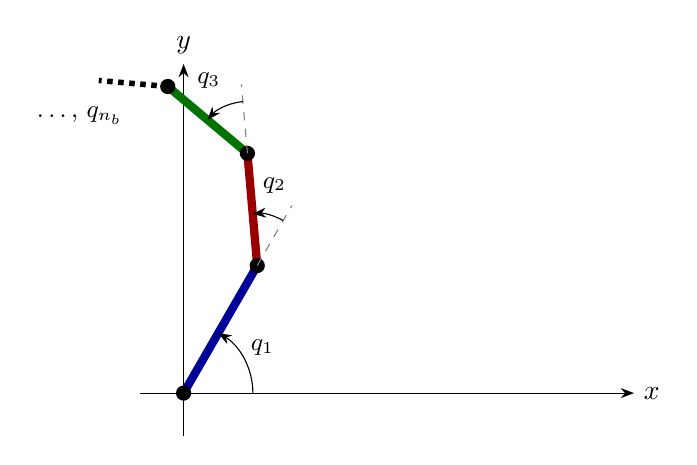
\begin{tikzpicture}[>=Stealth,scale=1.1]
  \draw[->] (-0.5,0) -- (5.2,0) node[right] {$x$};
  \draw[->] (0,-0.5) -- (0,3.8) node[above] {$y$};
  \coordinate (O) at (0,0);
  \coordinate (J1) at (60:1.7);
  \coordinate (J2) at ($(J1)+(95:1.3)$);
  \coordinate (J3) at ($(J2)+(140:1.2)$);
  \draw[line width=3pt,blue!60!black] (O) -- (J1);
  \draw[line width=3pt,red!60!black] (J1) -- (J2);
  \draw[line width=3pt,green!45!black] (J2) -- (J3);
  \draw[line width=2pt,dotted] (J3) -- ($(J3)+(175:0.8)$);
  \foreach \p in {O,J1,J2,J3} \fill (\p) circle (2.5pt);
  % angle arcs
  \draw[->] (0.8,0) arc (0:60:0.8); \node at (30:1.05) {\small $q_1$};
  \draw[dashed,gray] (J1) -- ($(J1)+(60:0.8)$);
  \draw[->] ($(J1)+(60:0.6)$) arc (60:95:0.6); \node at ($(J1)+(78:0.95)$) {\small $q_2$};
  \draw[dashed,gray] (J2) -- ($(J2)+(95:0.8)$);
  \draw[->] ($(J2)+(95:0.6)$) arc (95:140:0.6); \node at ($(J2)+(118:0.95)$) {\small $q_3$};
  \node at (-1.2,3.2) {\small \dots, $q_{n_b}$};
\end{tikzpicture}
\caption{Planar manipulator with $n_b$ links: one joint angle $q_i$ per joint.}
\end{figure}

\begin{intuition}
Imagine gluing the links together at the joints. Each glued joint removes two ``free sliding'' directions. Three links loose in the plane would have $9$ degrees of freedom; pin them into a chain anchored at the base and only $3$ remain: the three joint angles. The number of angles $=$ the number of joints.
\end{intuition}

\begin{proposition}\label{prop:so2-not-so3}
For three revolute joints, $\C=\SO(2)\times\SO(2)\times\SO(2)$, which is very different from $\SO(3)$: the two spaces have the same dimension $3$ but different topology.
\end{proposition}

\begin{intuition}
$\SO(3)$ describes all orientations of \emph{one} rigid body (roll, pitch, yaw). Three planar joints are three \emph{independent} angles each living on its own circle; they cannot all mix into one 3D rotation. Same number of parameters, different shape: it is the shape (topology), not just the count, that matters later.
\end{intuition}

\subsection{Spatial manipulator with $n_b$ links}

\begin{proposition}[Degrees of freedom of a spatial serial arm]
A spatial arm with $n_b$ links and $n_b$ revolute joints in $\W=\R^3$ has
\[
  6n_b-5n_b=n_b
\]
degrees of freedom: each link has $6$ degrees of freedom, but a revolute joint imposes $5$ constraints ($3$ positions and $2$ orientations are fixed; only rotation about the joint axis remains).
\end{proposition}

Even though the manipulator is spatial, each joint has a \emph{planar} orientation (a single angle), so again
\[
  \C=\SO(2)\times\dots\times\SO(2)=\SO(2)^{n_b}\qquad(n_b\text{ times}).
\]

\begin{intuition}
A hinge (revolute joint) always allows exactly one motion: turning about its axis. Whether the world is 2D or 3D, that one motion is a single angle. The ambient dimension changes the \emph{constraint count} ($2$ vs.\ $5$) but not the end result: one angle per joint.
\end{intuition}

% =====================================================================
\section{Topology of $\C$}\label{sec:topology}\pts{5--6}
% =====================================================================

\subsection{The problem with a flat picture of the 2R robot}

Take the 2R planar robot, $\C=\SO(2)\times\SO(2)$, $q=(q_1,q_2)^\top$. Since angles are periodic, $q_1$ and $q_1+2\pi$ give the \emph{same posture}. So if we naively draw $\C$ as the plane $\R^2$ of angle pairs, then two different points give the same posture: the map from this plane to postures is \emph{not injective}, which is bad for us.

\begin{figure}[ht]
\centering
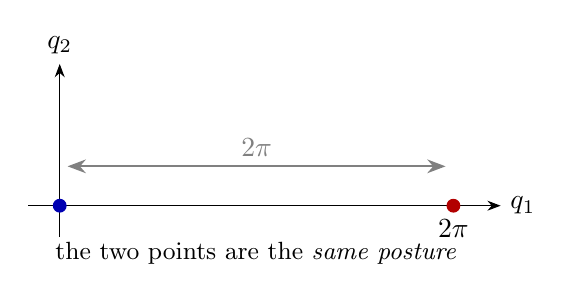
\begin{tikzpicture}[>=Stealth]
  \draw[->] (-0.4,0) -- (5.6,0) node[right] {$q_1$};
  \draw[->] (0,-0.4) -- (0,1.8) node[above] {$q_2$};
  \fill[blue!70!black] (0,0) circle (2.5pt);
  \fill[red!70!black] (5,0) circle (2.5pt);
  \draw[<->,thick,gray] (0.1,0.5) -- (4.9,0.5) node[midway,above] {$2\pi$};
  \node[below] at (5,-0.05) {$2\pi$};
  \node at (2.5,-0.6) {\small the two points are the \emph{same posture}};
\end{tikzpicture}
\caption{On the plane of angle pairs, $q_1=0$ and $q_1=2\pi$ (same $q_2$) correspond to the same posture: the map to postures is many-to-one.}
\end{figure}

A new attempt: restrict each angle to $[0,2\pi)$, i.e.\ draw $\C$ as the square $[0,2\pi)\times[0,2\pi)$. Now the correspondence with postures is one-to-one (considering only the two ``bad sides'' of the square, $q=0$ and $q=2\pi$, as the same). But this is still not good enough: two configurations $q_a$ and $q_b$ that are almost the same posture (one just below $2\pi$, the other just above $0$) look \emph{far apart} in the square.

\begin{figure}[ht]
\centering
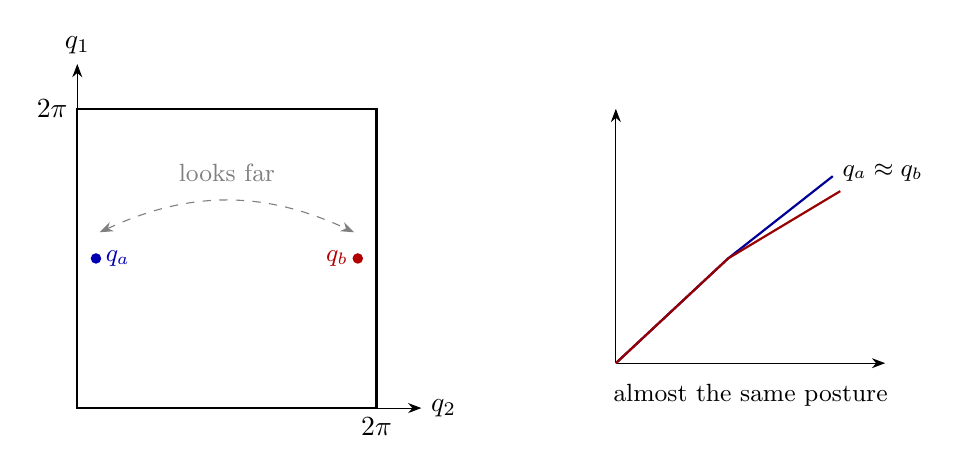
\begin{tikzpicture}[>=Stealth,scale=0.95]
  % square
  \draw[->] (0,0) -- (4.6,0) node[right] {$q_2$};
  \draw[->] (0,0) -- (0,4.6) node[above] {$q_1$};
  \draw[thick] (0,0) rectangle (4,4);
  \node[below] at (4,0) {$2\pi$};
  \node[left] at (0,4) {$2\pi$};
  \fill[blue!70!black] (0.25,2) circle (2pt) node[right] {\small $q_a$};
  \fill[red!70!black]  (3.75,2) circle (2pt) node[left] {\small $q_b$};
  \draw[<->,gray,dashed] (0.3,2.35) to[bend left=25] (3.7,2.35);
  \node[gray] at (2,3.15) {\small looks far};
  % posture plot
  \begin{scope}[shift={(7.2,0.6)}]
    \draw[->] (0,0) -- (3.6,0);
    \draw[->] (0,0) -- (0,3.4);
    \draw[thick,blue!60!black] (0,0) -- (1.5,1.4) -- (2.9,2.5);
    \draw[thick,red!60!black]  (0,0) -- (1.5,1.4) -- (3.0,2.3);
    \node[right] at (2.9,2.55) {\small $q_a\approx q_b$};
    \node[below] at (1.8,-0.15) {\small almost the same posture};
  \end{scope}
\end{tikzpicture}
\caption{The square picture of $\C$: $q_a$ and $q_b$ are close as postures but far in the flat picture.}
\end{figure}

So this topology does not describe exactly what is happening.

\subsection{Wrapping the space: the torus}

The fix is to \emph{wrap} the space: identify the opposite sides of the square (left with right, bottom with top) and embed the resulting 2D object in 3D. We obtain a \emph{torus} (from Latin, ``pillow'').

\begin{figure}[ht]
\centering
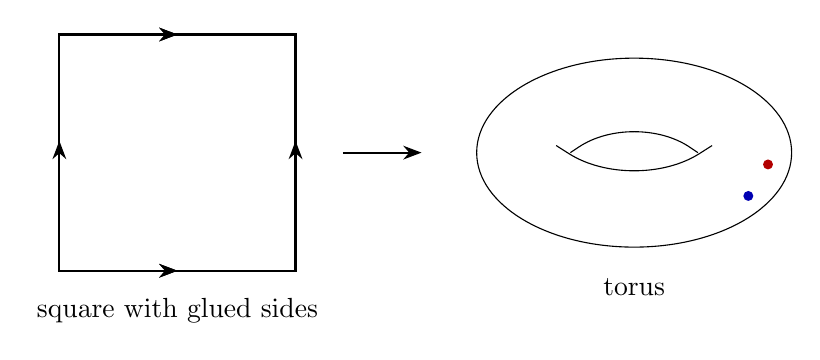
\begin{tikzpicture}[>=Stealth,scale=1]
  % identification square
  \begin{scope}
    \draw[thick] (0,0) rectangle (3,3);
    % vertical sides: single arrow, same direction
    \draw[thick,decoration={markings,mark=at position 0.55 with {\arrow{Stealth}}},postaction={decorate}] (0,0) -- (0,3);
    \draw[thick,decoration={markings,mark=at position 0.55 with {\arrow{Stealth}}},postaction={decorate}] (3,0) -- (3,3);
    % horizontal sides: double arrow
    \draw[thick,decoration={markings,mark=at position 0.5 with {\arrow{Stealth}\arrow{Stealth}}},postaction={decorate}] (0,0) -- (3,0);
    \draw[thick,decoration={markings,mark=at position 0.5 with {\arrow{Stealth}\arrow{Stealth}}},postaction={decorate}] (0,3) -- (3,3);
    \node at (1.5,-0.5) {square with glued sides};
  \end{scope}
  \draw[->,thick] (3.6,1.5) -- (4.6,1.5);
  % torus
  \begin{scope}[shift={(7.3,1.5)}]
    \draw (0,0) ellipse (2 and 1.2);
    \begin{scope}[scale=0.9]
      \path[rounded corners=24pt] (-.9,0)--(0,.6)--(.9,0) (-.9,0)--(0,-.56)--(.9,0);
      \draw[rounded corners=28pt] (-1.1,.1)--(0,-.6)--(1.1,.1);
      \draw[rounded corners=24pt] (-.9,0)--(0,.6)--(.9,0);
    \end{scope}
    \fill[blue!70!black] (1.45,-0.55) circle (1.8pt);
    \fill[red!70!black]  (1.7,-0.15) circle (1.8pt);
    \node at (0,-1.7) {torus};
  \end{scope}
\end{tikzpicture}
\caption{Gluing opposite sides of the square gives a torus. Points that were far apart in the square (across the seam) become neighbours on the torus.}
\end{figure}

\begin{proposition}
$\SO(2)\cong\Sph^1$ (the circle), hence the configuration space of the 2R planar robot is $\Sph^1\times\Sph^1=\mathbb{T}^2$, the torus, and in general $\SO(2)^{n_b}\cong\mathbb{T}^{n_b}$ is an $n_b$-dimensional torus.
\end{proposition}

\begin{intuition}
A joint angle is like a clock hand: after $2\pi$ you are back where you started, so one angle lives on a \emph{circle}, not on a line. Two joints give two circles, and a product of two circles is the surface of a doughnut. Walking off the right side of the square and reappearing on the left is just going around the doughnut the short way.
\end{intuition}

\subsection{Manifolds}

\begin{definition}[Manifold]
A \emph{manifold} of dimension $n$ is a space in which the neighbourhood of each point ``looks like'' a neighbourhood of $\R^n$. (For the torus, $\R^2$.)
\end{definition}

\begin{proposition}
Configuration spaces are manifolds (in general \emph{not} Euclidean anymore): $\R^m$, $\SO(2)$, $\SO(3)$, $\SE(2)$, $\SE(3)$ and their products are all manifolds.
\end{proposition}

\begin{intuition}
The Earth is the classical example: it is a sphere, yet a small enough patch looks flat, so a city map works. Locally we can use ordinary coordinates and calculus; globally the space can wrap around, and that is what a flat picture cannot show.
\end{intuition}

\begin{figure}[ht]
\centering
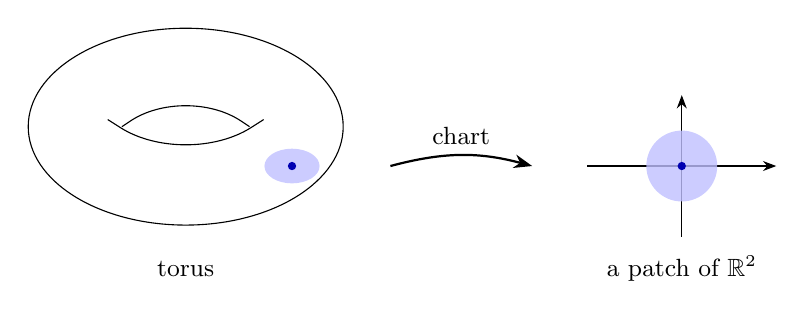
\begin{tikzpicture}[>=Stealth]
  \begin{scope}
    \draw (0,0) ellipse (2 and 1.25);
    \begin{scope}[scale=0.9]
    \path[rounded corners=24pt] (-.9,0)--(0,.6)--(.9,0) (-.9,0)--(0,-.56)--(.9,0);
    \draw[rounded corners=28pt] (-1.1,.1)--(0,-.6)--(1.1,.1);
    \draw[rounded corners=24pt] (-.9,0)--(0,.6)--(.9,0);
    \end{scope}
    \fill[blue!25,opacity=.8] (1.35,-0.5) ellipse (0.35 and 0.22);
    \fill[blue!70!black] (1.35,-0.5) circle (1.5pt);
    \node at (0,-1.8) {\small torus};
  \end{scope}
  \draw[->,thick] (2.6,-0.5) to[bend left=15] node[above] {\small chart} (4.4,-0.5);
  \begin{scope}[shift={(6.3,-0.5)}]
    \draw[->] (-1.2,0) -- (1.2,0);
    \draw[->] (0,-0.9) -- (0,0.9);
    \fill[blue!25,opacity=.8] (0,0) circle (0.45);
    \fill[blue!70!black] (0,0) circle (1.5pt);
    \node at (0,-1.3) {\small a patch of $\R^2$};
  \end{scope}
\end{tikzpicture}
\caption{A small neighbourhood of any point of the torus can be flattened (charted) onto a neighbourhood in $\R^2$: this is what ``looks like $\R^n$'' means.}
\end{figure}

% =====================================================================
\section{Distances in $\C$}\pts{6--8}
% =====================================================================

\subsection{What a distance must satisfy}

\begin{definition}[Distance (metric)]
A function $d:\C\times\C\to\R$ is a \emph{distance} if for all $q_A,q_B,q_C\in\C$:
\begin{enumerate}[nosep,label=(\roman*)]
  \item $d(q_A,q_B)\ge 0$;
  \item $d(q_A,q_B)=0$ if and only if $q_A=q_B$;
  \item $d(q_A,q_B)=d(q_B,q_A)$ (symmetry);
  \item $d(q_A,q_B)\le d(q_A,q_C)+d(q_C,q_B)$ (triangle inequality).
\end{enumerate}
\end{definition}


\begin{figure}[ht]
\centering
\begin{tikzpicture}[>=Stealth]
  \draw[->] (0,0) -- (0,3.2);
  \draw[->] (0,0) -- (3.4,-0.5);
  \draw[->] (0,0) -- (-1.5,-1.2);
  \node at (1.2,3.0) {$\C$};
  \coordinate (A) at (0.6,1.0);
  \coordinate (B) at (2.3,1.6);
  \fill[blue!70!black] (A) circle (2pt) node[left] {$q_A$};
  \fill[red!70!black] (B) circle (2pt) node[right] {$q_B$};
  \draw[green!45!black,very thick] (A) to[bend left=25] node[above] {$d(q_A,q_B)$} (B);
\end{tikzpicture}
\caption{The distance $d(q_A,q_B)$ between two points of the configuration space.}
\end{figure}

\subsection{Distances on manifolds and geodesics}

The classic (Euclidean) distance completely ignores the curvature of the space: for two points on a torus, the straight segment between them passes \emph{through the hole}, outside the manifold. So we cannot use the Euclidean distance.

\begin{figure}[ht]
\centering
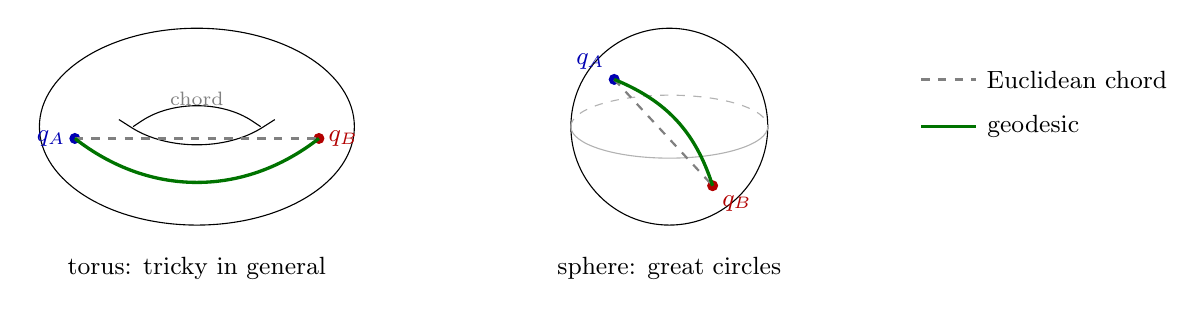
\begin{tikzpicture}[>=Stealth]
  % torus panel
  \begin{scope}
    \draw (0,0) ellipse (2 and 1.25);
    \begin{scope}[scale=0.9]
    \path[rounded corners=24pt] (-.9,0)--(0,.6)--(.9,0) (-.9,0)--(0,-.56)--(.9,0);
    \draw[rounded corners=28pt] (-1.1,.1)--(0,-.6)--(1.1,.1);
    \draw[rounded corners=24pt] (-.9,0)--(0,.6)--(.9,0);
    \end{scope}
    \fill[blue!70!black] (-1.55,-0.15) circle (2pt) node[left] {\small $q_A$};
    \fill[red!70!black]  (1.55,-0.15) circle (2pt) node[right] {\small $q_B$};
    \draw[dashed,gray,thick] (-1.55,-0.15) -- (1.55,-0.15);
    \draw[green!45!black,very thick] (-1.55,-0.15) to[bend right=38] (1.55,-0.15);
    \node at (0,-1.8) {\small torus: tricky in general};
    \node[gray,font=\scriptsize] at (0,0.35) {chord};
  \end{scope}
  % sphere panel
  \begin{scope}[shift={(6,0)}]
    \draw (0,0) circle (1.25);
    \draw[gray!60] (-1.25,0) arc (180:360:1.25 and 0.4);
    \draw[gray!60,dashed] (-1.25,0) arc (180:0:1.25 and 0.4);
    \fill[blue!70!black] (-0.7,0.6) circle (2pt) node[above left] {\small $q_A$};
    \fill[red!70!black]  (0.55,-0.75) circle (2pt) node[below right] {\small $q_B$};
    \draw[dashed,gray,thick] (-0.7,0.6) -- (0.55,-0.75);
    \draw[green!45!black,very thick] (-0.7,0.6) to[bend left=25] (0.55,-0.75);
    \node at (0,-1.8) {\small sphere: great circles};
  \end{scope}
  % legend
  \draw[dashed,gray,thick] (9.2,0.6) -- (9.9,0.6) node[right,black] {\small Euclidean chord};
  \draw[green!45!black,very thick] (9.2,0) -- (9.9,0) node[right,black] {\small geodesic};
\end{tikzpicture}
\caption{The chord between two points leaves the manifold (it crosses the hole of the torus, or the inside of the sphere); the geodesic stays on the surface. On a sphere the geodesic is an arc of a great circle; on a general manifold it is hard to compute.}
\end{figure}

\begin{definition}[Geodesic]
A \emph{geodesic} is a minimum-length path between two points \emph{on the manifold}. The geodesic distance is the length of that path.
\end{definition}

\begin{intuition}
For two cities on Earth, the geodesic is the great-circle route an aircraft follows, not the tunnel through the Earth. Geodesics are the ``honest'' distances on a curved space.
\end{intuition}

\subsection{The displacement metric}

Geodesics are easy on a sphere but can be tricky in general (and on a torus). Because of this difficulty, roboticists do not use them. They use instead a \emph{displacement metric}.

Let $p$ denote a point of the robot (e.g.\ the centre of mass, or the end point of a link), and $p(q)$ its position in $\W$ when the configuration is $q$.

\begin{definition}[Displacement metric]
\[
  d(q_A,q_B)=\max_{p\in\text{robot}}\ \norm{p(q_A)-p(q_B)} .
\]
It is the \emph{maximum displacement} of the points of the robot when moving from $q_A$ to $q_B$.
\end{definition}

\begin{proposition}
The displacement metric satisfies the four axioms of a distance (provided distinct configurations give distinct postures, which is the case for a minimal parametrization).
\end{proposition}

\begin{proof}
(i),(iii) hold because a norm is non-negative and symmetric, and the maximum of such quantities is too. (ii) If $q_A=q_B$ every point has zero displacement, so $d=0$; conversely $d=0$ means every point is at the same place in the two configurations, i.e.\ the postures coincide, hence $q_A=q_B$. (iv) For every point $p$,
\[
 \norm{p(q_A)-p(q_B)}\le\norm{p(q_A)-p(q_C)}+\norm{p(q_C)-p(q_B)}\le d(q_A,q_C)+d(q_C,q_B);
\]
taking the maximum over $p$ on the left gives the claim. \qedhere
\end{proof}

\begin{intuition}
Instead of measuring a length \emph{inside} the curved configuration space, we go back to the physical world and ask: ``how far does the worst-behaved point of the robot have to travel?'' We use ordinary Euclidean distances there, where they are perfectly fine, and the curvature of $\C$ takes care of itself. Nice side effect: this measure is automatically periodic, since $q_1$ and $q_1+2\pi$ give the same positions.
\end{intuition}

\begin{example}[1R robot]
A single link of length $L$ rotating about the origin; $q_A$, $q_B$ are two angles differing by $\Delta\in[0,\pi]$. A point at distance $r\le L$ from the joint moves by the chord $2r\sin(\Delta/2)$, largest at the tip, so
\[
  d(q_A,q_B)=2L\sin\!\big(\tfrac{\Delta}{2}\big).
\]
We are effectively using the \emph{Euclidean} distance between the two tip positions to measure distance on the manifold.
\end{example}

\begin{figure}[ht]
\centering
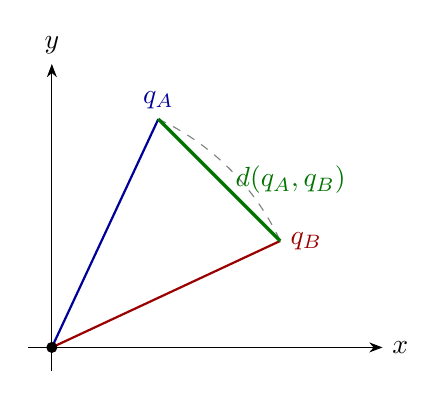
\begin{tikzpicture}[>=Stealth]
  \draw[->] (-0.3,0) -- (4.2,0) node[right] {$x$};
  \draw[->] (0,-0.3) -- (0,3.6) node[above] {$y$};
  \coordinate (O) at (0,0);
  \coordinate (A) at (65:3.2);
  \coordinate (B) at (25:3.2);
  \draw[thick,blue!60!black] (O) -- (A) node[above] {$q_A$};
  \draw[thick,red!60!black] (O) -- (B) node[right] {$q_B$};
  \draw[dashed,gray] (65:3.2) arc (65:25:3.2);
  \draw[very thick,green!45!black] (A) -- (B) node[midway,right=2pt] {$d(q_A,q_B)$};
  \fill (O) circle (2pt);
\end{tikzpicture}
\caption{1R robot: the displacement metric is the Euclidean distance between the tip in the two configurations.}
\end{figure}

\begin{example}[Numbers for the 1R robot, $L=1$]
For $\Delta=\pi/2$: $d=2\sin(\pi/4)=\sqrt2\approx1.41$. For two angles that differ by $2\pi-0.1$ (almost a full turn): the wrapped difference is $0.1$, so $d=2\sin(0.05)\approx0.10$ -- correctly tiny, whereas the flat difference of angles ($6.18$) would call them far apart.
\end{example}

\begin{figure}[ht]
\centering
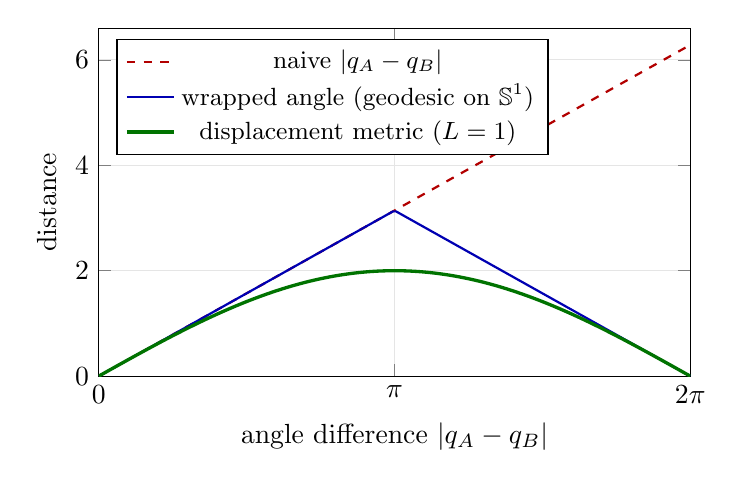
\begin{tikzpicture}
\begin{axis}[width=0.75\linewidth,height=6cm,
  xlabel={angle difference $|q_A-q_B|$},ylabel={distance},
  xmin=0,xmax=2*pi,ymin=0,ymax=6.6,
  xtick={0,pi,2*pi},xticklabels={$0$,$\pi$,$2\pi$},
  trig format plots=rad,legend pos=north west,legend style={font=\small},
  grid=both,grid style={gray!20}]
\addplot[dashed,red!70!black,thick,domain=0:2*pi,samples=100] {x};
\addlegendentry{naive $|q_A-q_B|$}
\addplot[blue!70!black,thick,domain=0:2*pi,samples=200] {min(x,2*pi-x)};
\addlegendentry{wrapped angle (geodesic on $\Sph^1$)}
\addplot[green!45!black,very thick,domain=0:2*pi,samples=200] {2*sin(x/2)};
\addlegendentry{displacement metric ($L=1$)}
\end{axis}
\end{tikzpicture}
\caption{Three ways to measure the distance between two configurations of a 1R robot. The naive difference grows up to $2\pi$; the other two vanish again at $2\pi$ because the configuration wraps around.}
\end{figure}

\begin{example}[2R robot]
With two links we take the maximum over the points of both links. The displacement of a point on a link is an affine function of its position along the link, so its norm is convex and the maximum is attained at a link endpoint: the base (which never moves), the elbow joint, or the tip. In Figure~\ref{fig:2R-disp} (link lengths $1.6$ and $1$) the tip moves by about $0.64$ but the elbow moves by about $1.60$, so $d(q_A,q_B)\approx1.60$: the maximum is \emph{not} necessarily at the tip.
\end{example}

\begin{figure}[ht]
\centering
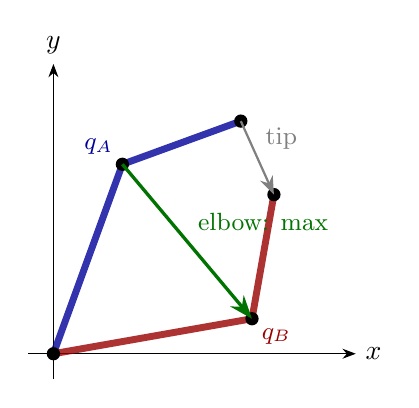
\begin{tikzpicture}[>=Stealth,scale=1.6]
  \draw[->] (-0.2,0) -- (2.4,0) node[right] {$x$};
  \draw[->] (0,-0.2) -- (0,2.3) node[above] {$y$};
  \coordinate (O) at (0,0);
  \coordinate (JA) at (70:1.6);
  \coordinate (EA) at ($(JA)+(20:1)$);
  \coordinate (JB) at (10:1.6);
  \coordinate (EB) at ($(JB)+(80:1)$);
  \draw[line width=2.5pt,blue!60!black,opacity=.8] (O) -- (JA) -- (EA);
  \draw[line width=2.5pt,red!60!black,opacity=.8] (O) -- (JB) -- (EB);
  \fill (O) circle (1.5pt);
  \fill (JA) circle (1.5pt); \fill (EA) circle (1.5pt);
  \fill (JB) circle (1.5pt); \fill (EB) circle (1.5pt);
  \node[blue!60!black,above left] at (JA) {\small $q_A$};
  \node[red!60!black,below right] at (JB) {\small $q_B$};
  \draw[->,very thick,green!45!black] (JA) -- (JB) node[midway,above right] {\small elbow: max};
  \draw[->,thick,gray] (EA) -- (EB) node[midway,above right=-1pt] {\small tip};
\end{tikzpicture}
\caption{2R robot in two configurations. The displacement of each characteristic point is drawn; the displacement metric takes the largest one (here the elbow).}
\label{fig:2R-disp}
\end{figure}

\begin{figure}[ht]
\centering
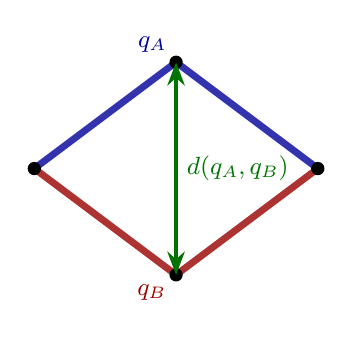
\begin{tikzpicture}[>=Stealth,scale=1.5]
  \coordinate (O) at (0,0);
  \coordinate (E1) at (1.2,0.9);
  \coordinate (E2) at (1.2,-0.9);
  \coordinate (T) at (2.4,0);
  \draw[line width=2.5pt,blue!60!black,opacity=.8] (O) -- (E1) -- (T);
  \draw[line width=2.5pt,red!60!black,opacity=.8] (O) -- (E2) -- (T);
  \foreach \p in {O,E1,E2,T} \fill (\p) circle (1.6pt);
  \draw[<->,very thick,green!45!black] (E1) -- (E2) node[midway,right] {\small $d(q_A,q_B)$};
  \node[blue!60!black,above left] at (E1) {\small $q_A$};
  \node[red!60!black,below left] at (E2) {\small $q_B$};
\end{tikzpicture}
\caption{2R robot with equal links, "elbow up" vs "elbow down", same tip: the tip does not move, and the displacement metric equals the distance between the two elbows.}
\end{figure}

\subsection{The max over infinitely many points}

There is a catch: the definition asks for a maximum over an \emph{infinite} set of points. Intuitively, for polygonal robots we should only look at the \emph{vertices}, but it is not always like this.

\begin{proposition}
If the robot is a convex polygon (or a union of segments, as a chain of links), the maximum in the displacement metric is attained at a vertex (link endpoint).
\end{proposition}

\begin{proof}
Under a rigid motion, the position of a body point $r$ is affine in $r$, so $r\mapsto p(q_A)-p(q_B)$ is affine on the body. The norm of an affine function is convex, and a convex function on a polytope attains its maximum at a vertex.
\end{proof}

\begin{intuition}
The point that moves most is the one sticking out the farthest -- a corner, or the tip of a link. For a curved body (e.g.\ a disk with attached parts) there is no finite list of corners to check, so we need an approximation.
\end{intuition}

\subsection{A practical alternative: control points}

We can use a predetermined number of points, called \emph{control points}, which, if chosen correctly, give a good approximation.

\begin{definition}[Control-point distance]
Fix control points $\{p_1,p_2,\dots,p_c\}$ on the robot. Define
\[
  d(q_A,q_B)=\sum_{i=1}^{c}\norm{p_i(q_A)-p_i(q_B)} .
\]
\end{definition}

\begin{algorithm}[Computing the control-point distance]
\begin{enumerate}[nosep]
  \item Choose $c$ representative points $p_1,\dots,p_c$ on the robot (e.g.\ centre of mass, link endpoints).
  \item For each $i$, compute the forward kinematics $p_i(q_A)$ and $p_i(q_B)$.
  \item Return $\sum_{i=1}^c\norm{p_i(q_A)-p_i(q_B)}$.
\end{enumerate}
\end{algorithm}

\begin{figure}[ht]
\centering
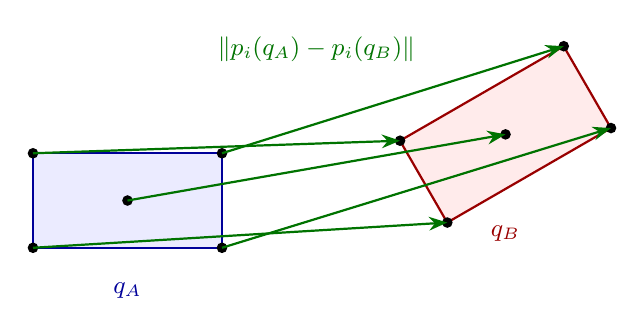
\begin{tikzpicture}[>=Stealth,scale=1.2]
  \begin{scope}[shift={(0,0)}]
    \coordinate (a1) at (-1,-.5); \coordinate (a2) at (1,-.5);
    \coordinate (a3) at (1,.5);   \coordinate (a4) at (-1,.5); \coordinate (a5) at (0,0);
    \draw[thick,blue!60!black,fill=blue!8] (a1) rectangle (a3);
  \end{scope}
  \begin{scope}[shift={(4,0.7)},rotate=30]
    \coordinate (b1) at (-1,-.5); \coordinate (b2) at (1,-.5);
    \coordinate (b3) at (1,.5);   \coordinate (b4) at (-1,.5); \coordinate (b5) at (0,0);
    \draw[thick,red!60!black,fill=red!8] (b1) rectangle (b3);
  \end{scope}
  \foreach \i in {1,2,3,4,5}{
    \fill (a\i) circle (1.6pt);
    \fill (b\i) circle (1.6pt);
    \draw[->,green!45!black,thick] (a\i) -- (b\i);
  }
  \node[blue!60!black] at (0,-0.95) {\small $q_A$};
  \node[red!60!black] at (4,-0.35) {\small $q_B$};
  \node[green!45!black,font=\small] at (2,1.6) {$\norm{p_i(q_A)-p_i(q_B)}$};
\end{tikzpicture}
\caption{Control points $p_1,\dots,p_5$ (four corners and the centre) of a rectangular robot. The distance is the sum of the lengths of the displacement arrows.}
\end{figure}

\begin{proposition}
The control-point distance is symmetric and satisfies the triangle inequality. It is a genuine distance if the control points are chosen so that $p_i(q_A)=p_i(q_B)$ for all $i$ implies $q_A=q_B$; otherwise it is only a pseudo-distance.
\end{proposition}

\begin{proof}
Each summand is a norm of a difference, so symmetry holds, and the triangle inequality holds termwise and is preserved by the sum. The condition on control points gives axiom (ii). 
\end{proof}

\begin{intuition}
Rather than tracking every point, you pin a few ``sensors'' on the robot (say, the tip and the middle) and add up how far they each move. A moving robot cannot fool three well-placed sensors: if they all end up in the same places, the robot is in the same pose. The cost: an approximation of the true worst-case displacement, but cheap and easy to differentiate.
\end{intuition}

% =====================================================================
\section{Summary}
% =====================================================================

\subsection{Configuration spaces seen in this lecture}

\begin{center}
\renewcommand{\arraystretch}{1.25}
\begin{tabular}{@{}llcc@{}}
\toprule
Robot & $\C$ & $n=\dim\C$ & Euclidean? \\
\midrule
Point in $\R^3$ & $\R^3$ & 3 & yes \\
Disk in $\R^2$ & $\R^2$ & 2 & yes \\
Disk with tick / polygon in $\R^2$ & $\SE(2)=\R^2\times\SO(2)$ & 3 & no \\
Polyhedron in $\R^3$ & $\SE(3)=\R^3\times\SO(3)$ & 6 & no \\
Planar $n_b$-R arm & $\SO(2)^{n_b}=\mathbb{T}^{n_b}$ & $n_b$ & no \\
Spatial $n_b$-R arm & $\SO(2)^{n_b}=\mathbb{T}^{n_b}$ & $n_b$ & no \\
\bottomrule
\end{tabular}
\end{center}

\subsection{Distances on $\C$}

\begin{center}
\renewcommand{\arraystretch}{1.25}
\begin{tabular}{@{}p{3.3cm}p{4.2cm}p{4.6cm}@{}}
\toprule
Distance & Definition & Pros / cons \\
\midrule
Euclidean in parameters & $\norm{q_A-q_B}$ & simple, but ignores wrapping (bad on angles) \\
Geodesic & shortest path on the manifold & exact, but hard to compute in general \\
Displacement metric & $\max_p\norm{p(q_A)-p(q_B)}$ & respects topology, physically meaningful; max over infinitely many points \\
Control points & $\sum_i\norm{p_i(q_A)-p_i(q_B)}$ & cheap approximation; needs well-chosen points \\
\bottomrule
\end{tabular}
\end{center}

\subsection{Key take-aways}

\begin{itemize}
  \item The configuration space $\C$ is the space of all values of a \emph{minimal} set of parameters describing the robot; in it the robot is a single point, and planning/control become problems about that point.
  \item Joints reduce degrees of freedom: a planar arm has $3n_b-2n_b=n_b$ and a spatial arm $6n_b-5n_b=n_b$ degrees of freedom -- one angle per joint.
  \item Because angles are periodic, $\C$ is generally a \emph{manifold} (e.g.\ a torus for a 2R arm), not $\R^n$: same dimension does not mean same shape ($\SO(2)^3\ne\SO(3)$).
  \item Euclidean distance in parameter space is misleading on a manifold; geodesics are correct but hard to compute.
  \item Roboticists use the \emph{displacement metric} (max point displacement) or its practical version with a few \emph{control points}.
\end{itemize}

\newpage

% ======================================================================
% Lecture 2
% ======================================================================
\part{Lecture 2}

\begin{tcolorbox}[colback=gray!5, colframe=black!40, boxrule=0.4pt, title={About these notes}, fonttitle=\bfseries, coltitle=black, colbacktitle=gray!15]
\small
These notes have two parts. \textbf{Part I} is based on the lecture slides (\texttt{WheeledMobileRobots1\_Slides.pdf}, slide ranges in parentheses). \textbf{Part II} is based on the second half of the lecture, provided as handwritten notes (\texttt{AMR02.pdf}, page ranges in parentheses). No companion book chapter was provided for either part, so the formal statements (Definitions, Propositions, Lemmas, Theorems, proofs) formalise the content of the slides/notes with standard results. Whatever is \emph{not} in the source is explicitly tagged \emph{(beyond the slides)} or \emph{(beyond the notes)}. In Part II I corrected a typo in the notes ($\partial h/\partial k$ read as $\partial h/\partial q$) and added the solution of the example left open on page 6. Red dashed or framed boxes marked ``Blank'' are spots for photographs/videos on the slides that were deliberately not redrawn; all other figures are original TikZ drawings.
\end{tcolorbox}
 
% =====================================================================
\part{Mechanics of Mobile Robots}
 
\section{Outline of this lecture \emph{(slides 1--2)}}
 
The lecture opens the part of the course on \emph{wheeled mobile robots} (WMRs). It covers four topics:
\begin{itemize}[nosep]
  \item \textbf{ground locomotion}: how a robot moves by contact with the ground;
  \item \textbf{balance}: what it takes for the robot not to fall;
  \item \textbf{wheels}: the three basic wheel types;
  \item \textbf{kinematic structures}: the classical ways of combining wheels on a chassis.
\end{itemize}
 
\begin{intuition}
Think of this lecture as the \emph{hardware vocabulary} of the course. Later lectures write equations of motion (kinematics, control) for each structure; to do so one first needs to know which wheel is where, which wheels are motorised, and which can steer. Everything here is about that bookkeeping.
\end{intuition}
 
% =====================================================================
\section{Ground locomotion \emph{(slide 3)}}

Moving on the ground requires \emph{contact} between the robot and the terrain. The slides distinguish two ways of establishing it.

\begin{definition}[Wheeled mobile robot]
A \emph{wheeled mobile robot} (WMR) typically consists of a single rigid body (the \emph{base} or \emph{chassis}) plus a set of wheels that connect it to the ground.
\end{definition}

\begin{definition}[Legged robot]
A \emph{legged robot} typically consists of \emph{several} rigid bodies articulated through joints; the contact with the ground is made through the feet.
\end{definition}

Some robots achieve ground locomotion with neither wheels nor feet, for instance \emph{snake robots}.

\begin{figure}[H]
\centering
\photobox{3.2cm}{wheeled: planetary rover}\hfill
\photobox{3.2cm}{legged: quadruped robot}\hfill
\photobox{3.2cm}{no wheels/feet: snake robot}
\caption{Photographs on slide 3 (not redrawn).}
\end{figure}

\begin{intuition}
The difference is in the \emph{mechanical complexity}: a WMR is one rigid body plus wheels, so its configuration is just the position and orientation of the chassis (plus steering angles); a legged robot is an articulated system, and every joint adds a degree of freedom to control. This is why the course starts with WMRs.
\end{intuition}

% =====================================================================
\section{Balance (not falling) \emph{(slides 4--5)}}

\subsection{Static balance and the support polygon}

\begin{definition}[Support polygon]
The \emph{support polygon} is the convex hull of the points where the robot touches the ground: the wheel contact points for a WMR, the footprints for a legged robot.
\end{definition}

\begin{definition}[Static balance]
A robot is \emph{statically balanced} when the vertical projection of its Center of Mass (CoM) on the ground falls inside the support polygon.
\end{definition}

\begin{figure}[H]
\centering
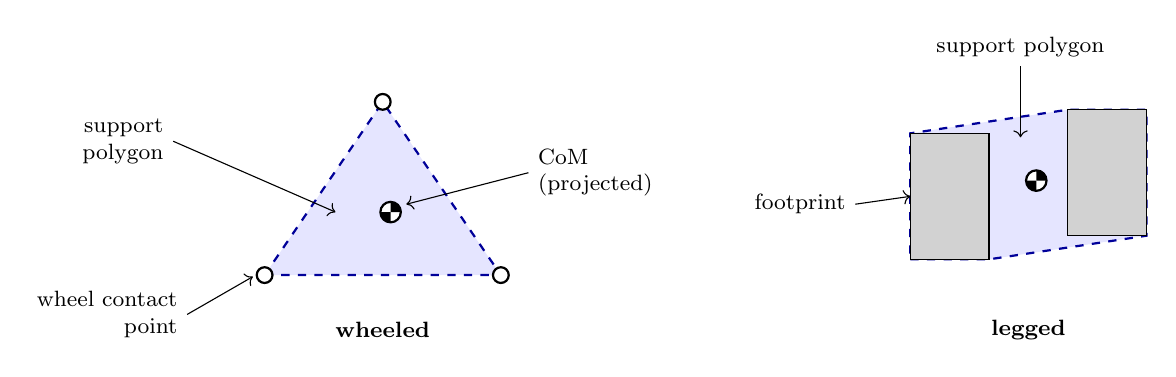
\begin{tikzpicture}[font=\footnotesize]
% wheeled
\fill[blue!10] (0,0)--(3,0)--(1.5,2.2)--cycle;
\draw[dashed,blue!60!black,thick] (0,0)--(3,0)--(1.5,2.2)--cycle;
\foreach \x/\y in {0/0,3/0,1.5/2.2} \draw[fill=white,thick] (\x,\y) circle (0.1);
\com{1.6,0.8}
\node at (1.5,-0.7) {\textbf{wheeled}};
\node[align=right] (a1) at (-1.8,1.7) {support\\polygon};
\draw[->] (a1.east)--(0.9,0.8);
\node[align=right] (a2) at (-2.0,-0.5) {wheel contact\\point};
\draw[->] (a2.east)--(-0.15,-0.02);
\node[align=left] (a3) at (4.2,1.3) {CoM\\(projected)};
\draw[->] (a3.west)--(1.8,0.9);
% legged
\begin{scope}[xshift=8.2cm]
\fill[blue!10] (0,0.2)--(1,0.2)--(3,0.5)--(3,2.1)--(2,2.1)--(0,1.8)--cycle;
\draw[dashed,blue!60!black,thick] (0,0.2)--(1,0.2)--(3,0.5)--(3,2.1)--(2,2.1)--(0,1.8)--cycle;
\draw[fill=gray!35] (0,0.2) rectangle (1,1.8);
\draw[fill=gray!35] (2,0.5) rectangle (3,2.1);
\com{1.6,1.2}
\node at (1.5,-0.7) {\textbf{legged}};
\node[align=right] (b1) at (-1.4,0.9) {footprint};
\draw[->] (b1.east)--(0,1.0);
\node[align=left] (b2) at (1.4,2.9) {support polygon};
\draw[->] (b2.south)--(1.4,1.75);
\end{scope}
\end{tikzpicture}
\caption{Support polygons (slide 4). Wheeled robot: triangle through three wheel contact points. Legged robot: convex hull of the two footprints. The projected CoM ($\otimes$-like symbol) must lie inside.}
\end{figure}

For WMRs the slides state a consequence: \emph{one needs 3 wheels}. Here is the formal reason.

\begin{proposition}[Three wheels are necessary]\label{prop:three}
A robot whose support polygon has non-empty interior needs at least three ground contact points that are not collinear. Consequently, a WMR that must be statically balanced with a robust margin needs at least 3 wheels.
\end{proposition}
\begin{proof}
The convex hull of one point is a point; of two points, a segment; of three or more collinear points, still a segment. All of these have empty interior in the plane, so the CoM projection can lie in them only by an unstable coincidence. Three non-collinear points span a triangle, which has non-empty interior.
\end{proof}

\begin{intuition}
A stool with one or two legs falls; a three-legged stool stands. With two wheels the robot can rotate about the line through the two contact points (like a seesaw), unless extra dynamic control is used. This is why the differential-drive robot of slide 9 adds a third, passive wheel (a caster) ``for balance''.
\end{intuition}

The support polygon also tells us how the weight is shared among the wheels.

% \begin{lemma}[Load distribution, three wheels \emph{(beyond the slides)}]\label{lem:load}
% Let the contact points $p_1,p_2,p_3\in\mathbb R^2$ be non-collinear, let $c\in\mathbb R^2$ be the projection of the CoM and $m$ the mass. In static equilibrium the vertical contact forces are $N_i=\lambda_i\,mg$, where $(\lambda_1,\lambda_2,\lambda_3)$ are the barycentric coordinates of $c$ with respect to the triangle, i.e.\ the unique solution of
% \[
% \lambda_1+\lambda_2+\lambda_3=1,\qquad \lambda_1p_1+\lambda_2p_2+\lambda_3p_3=c .
% \]
% Contacts can only push, so $N_i\ge 0$ for all $i$, i.e.\ $c$ lies in the (closed) triangle.
% \end{lemma}
% \begin{proof}
% Vertical equilibrium gives $\sum_i N_i=mg$. Balance of moments about the two horizontal axes gives $\sum_i N_ip_i=mg\,c$. Dividing by $mg$ these are exactly the barycentric equations. The coefficient matrix $\begin{bmatrix}1&1&1\\p_1&p_2&p_3\end{bmatrix}$ is invertible if and only if the points are not collinear, hence the solution is unique. If some $\lambda_i<0$ the ground would have to pull the wheel $i$: it lifts off and the robot tips over the opposite edge.
% \end{proof}

% \begin{algorithm}[Static balance test for a 3-wheeled robot \emph{(beyond the slides)}]
% Input: $p_1,p_2,p_3,c$.
% \begin{enumerate}[nosep]
%   \item Compute the signed area $A(a,b,d)=\tfrac12\det[\,b-a,\ d-a\,]$.
%   \item Set $\lambda_1=A(c,p_2,p_3)/A(p_1,p_2,p_3)$, $\lambda_2=A(p_1,c,p_3)/A(p_1,p_2,p_3)$, $\lambda_3=A(p_1,p_2,c)/A(p_1,p_2,p_3)$.
%   \item Return \textsc{balanced} if $\lambda_i>0$ for all $i$; otherwise \textsc{tips over}.
% \end{enumerate}
% \end{algorithm}

\begin{example}
A differential-drive robot has driving wheels at $p_1=(0,0.3)$, $p_2=(0,-0.3)$ and a caster at $p_3=(0.4,0)$ (metres), so $A(p_1,p_2,p_3)=0.12$\,m$^2$. With $c=(0.1,0.05)$ the algorithm gives $\lambda=(0.458,\,0.292,\,0.25)$: all positive, so the robot is balanced and the caster carries 25\% of the weight. After loading a payload that moves the CoM to $c=(0.3,0.1)$, we get $\lambda=(7/24,\,-1/24,\,3/4)$. Since $\lambda_2<0$, wheel~2 lifts and the robot tips over the edge $p_1p_3$.
\end{example}

% \begin{corollary}[Available traction \emph{(beyond the slides)}]
% If wheels 1 and 2 are the driven ones and $\mu$ is the Coulomb friction coefficient, the maximum total traction force is $F_{\max}=\mu(\lambda_1+\lambda_2)mg=\mu(1-\lambda_3)mg$.
% \end{corollary}
% \begin{proof}
% Each driven wheel can transmit at most $\mu N_i$ and $N_i=\lambda_i mg$ by Lemma~\ref{lem:load}.
% \end{proof}

\begin{intuition}
The weight splits among the wheels like a seesaw: the closer the CoM is to a wheel, the more load that wheel carries. In the example the caster carries a quarter of the weight, so 75\% of the weight presses on the driving wheels, which is what gives them traction. If the load moves far from the centre, one wheel is relieved of all weight and the robot tips. With four or more wheels the loads are no longer unique (like a four-legged table that wobbles on uneven ground), which is why real robots with more than three wheels need suspensions.
\end{intuition}

\subsection{Dynamic balance and the Zero Moment Point \emph{(slides 4--5)}}

\begin{definition}[Dynamic balance]
In \emph{dynamic balance}, the CoM in the static criterion is replaced by the \emph{Zero Moment Point} (ZMP), the point of the ground about which the horizontal components of the moment of gravity and inertial forces vanish. The robot is dynamically balanced when the ZMP lies inside the support polygon.
\end{definition}

% \begin{proposition}[ZMP of a point mass \emph{(beyond the slides)}]
% For a point mass at $(x_c,z_c)$ moving in the sagittal plane, the ZMP abscissa is
% \[
% x_{\mathrm{zmp}}=x_c-\frac{z_c}{g+\ddot z_c}\,\ddot x_c .
% \]
% \end{proposition}
% \begin{proof}
% Take moments about the ground point $(x_{\mathrm{zmp}},0)$. The vertical force $m(g+\ddot z_c)$ at $x_c$ contributes $m(g+\ddot z_c)(x_c-x_{\mathrm{zmp}})$, the horizontal inertia force contributes $-m\ddot x_c z_c$. Setting the sum to zero and solving gives the formula.
% \end{proof}

\begin{example}
With $z_c=0.8$\,m, $\ddot z_c=0$ and $\ddot x_c=1$\,m/s$^2$: $x_{\mathrm{zmp}}=x_c-0.8/9.81\approx x_c-8.2$\,cm. The ZMP lies 8.2\,cm behind the CoM projection.
\end{example}

\begin{figure}[H]
\centering
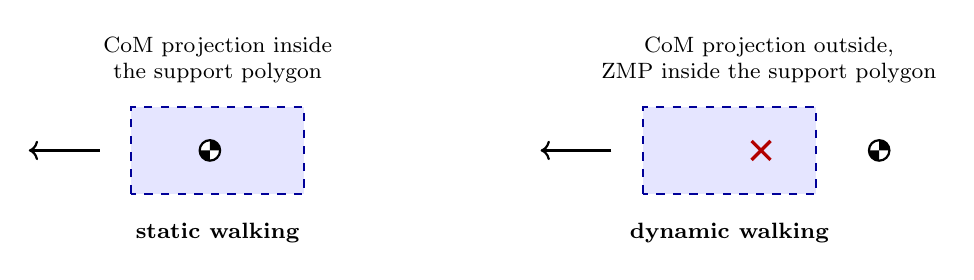
\begin{tikzpicture}[font=\footnotesize]
% static walking
\fill[blue!10] (0,0) rectangle (2.2,1.1);
\draw[thick,dashed,blue!60!black] (0,0) rectangle (2.2,1.1);
\com{1.0,0.55}
\node at (1.1,-0.5) {\textbf{static walking}};
\node[align=center] at (1.1,1.7) {CoM projection inside\\the support polygon};
% dynamic walking
\begin{scope}[xshift=6.5cm]
\fill[blue!10] (0,0) rectangle (2.2,1.1);
\draw[thick,dashed,blue!60!black] (0,0) rectangle (2.2,1.1);
\com{3.0,0.55}
\zmpmark{1.5,0.55}
\node at (1.1,-0.5) {\textbf{dynamic walking}};
\node[align=center] at (1.6,1.7) {CoM projection outside,\\ZMP inside the support polygon};
\draw[->,thick] (-0.4,0.55)--(-1.3,0.55) node[left]{};
\end{scope}
\draw[->,thick] (-0.4,0.55)--(-1.3,0.55);
\end{tikzpicture}
\caption{Static vs.\ dynamic walking (slide 5), shown for a single stance foot, top view. Arrows: walking direction. Red cross: ZMP.}
\end{figure}

\begin{intuition}
Carrying a tray while walking fast: you do not keep the tray's weight right above your feet, you lean and let motion help. Static walking is the cautious version, the CoM never leaves the foot area, so the robot could stop at any instant without falling; it is slow. In dynamic walking the CoM may be momentarily outside the foot, and the robot stays up because the accelerations move the ZMP back inside. The slide contrasts two humanoids walking one way or the other.
\end{intuition}

% =====================================================================
\section{Wheels: 3 basic types \emph{(slides 6--8)}}

Wheels are classified by how their orientation relates to the chassis and by whether they are motorised (\emph{active}) or free (\emph{passive}).

\subsection{Fixed wheel \emph{(slide 6)}}
\begin{definition}[Fixed wheel]
A wheel with \emph{fixed orientation} with respect to the chassis. It may be \emph{active} (used for driving) or \emph{passive} (used for balance).
\end{definition}

\subsection{Orientable (steerable) wheel \emph{(slide 7)}}
\begin{definition}[Orientable wheel]
A wheel whose orientation with respect to the chassis is \emph{variable}. It is typically \emph{active} (used for steering).
\end{definition}

\subsection{Caster wheel \emph{(slide 8)}}
\begin{definition}[Caster wheel]
A wheel with variable orientation with respect to the chassis, typically \emph{passive} (used for balance) but possibly active, that \emph{automatically aligns with the direction of motion}.
\end{definition}

\begin{figure}[H]
\centering
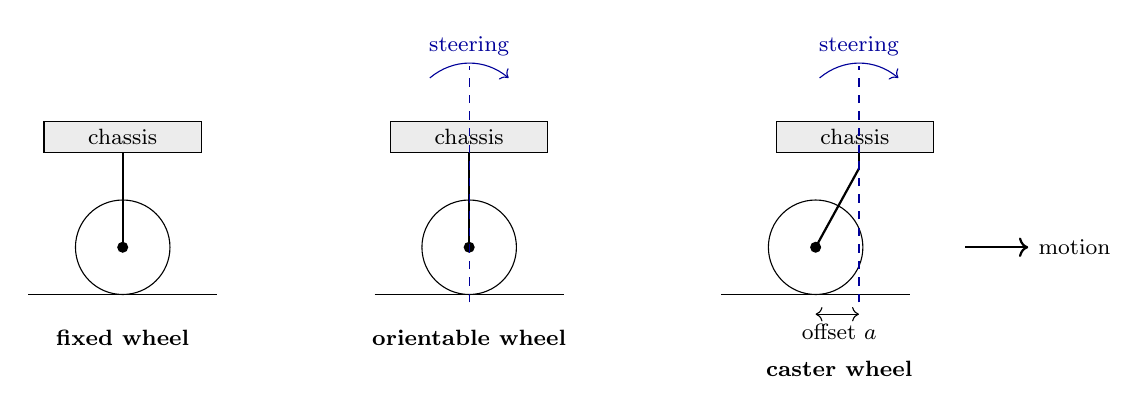
\begin{tikzpicture}[font=\footnotesize]
% fixed
\begin{scope}
\draw (-1.2,0)--(1.2,0);
\draw (0,0.6) circle (0.6); \fill (0,0.6) circle (2pt);
\draw[thick] (0,0.6)--(0,1.8);
\draw[fill=gray!15] (-1,1.8) rectangle (1,2.2); \node at (0,2.0) {chassis};
\node at (0,-0.55) {\textbf{fixed wheel}};
\end{scope}
% orientable
\begin{scope}[xshift=4.4cm]
\draw (-1.2,0)--(1.2,0);
\draw (0,0.6) circle (0.6); \fill (0,0.6) circle (2pt);
\draw[thick] (0,0.6)--(0,1.8);
\draw[fill=gray!15] (-1,1.8) rectangle (1,2.2); \node at (0,2.0) {chassis};
\draw[dashed,blue!60!black] (0,-0.1)--(0,2.9);
\draw[->,blue!60!black] (-0.5,2.75) to[bend left=40] (0.5,2.75);
\node[blue!60!black] at (0,3.15) {steering};
\node at (0,-0.55) {\textbf{orientable wheel}};
\end{scope}
% caster
\begin{scope}[xshift=8.8cm]
\draw (-1.2,0)--(1.2,0);
\draw (0,0.6) circle (0.6); \fill (0,0.6) circle (2pt);
\draw[thick] (0.55,1.6)--(0,0.6);
\draw[thick] (0.55,1.6)--(0.55,1.8);
\draw[fill=gray!15] (-0.5,1.8) rectangle (1.5,2.2); \node at (0.5,2.0) {chassis};
\draw[dashed,blue!60!black] (0.55,-0.1)--(0.55,2.9);
\draw[->,blue!60!black] (0.05,2.75) to[bend left=40] (1.05,2.75);
\node[blue!60!black] at (0.55,3.15) {steering};
\draw[<->] (0,-0.25)--(0.55,-0.25);
\node[below] at (0.3,-0.25) {offset $a$};
\draw[->,thick] (1.9,0.6)--(2.7,0.6) node[right]{motion};
\node at (0.3,-0.95) {\textbf{caster wheel}};
\end{scope}
\end{tikzpicture}
\caption{Side views of the three wheel types. The steering axis of the orientable wheel passes through the wheel centre; that of the caster is offset by a distance $a$, with the wheel trailing behind it.}
\end{figure}

\begin{table}[H]
\centering\small
\begin{tabular}{@{}lll@{}}
\toprule
Wheel & Orientation w.r.t.\ chassis & Typical role\\
\midrule
Fixed & constant & active (driving) or passive (balance)\\
Orientable & variable & active (steering)\\
Caster & variable, self-aligning & passive (balance), possibly active\\
\bottomrule
\end{tabular}
\caption{The three basic wheel types (slides 6--8).}
\end{table}

% \begin{proposition}[Self-alignment of a caster \emph{(beyond the slides)}]
% Let the pivot move with speed $v>0$ along a fixed direction of angle $\alpha$ and assume rolling without lateral slip. If $\varphi$ is the angle of the wheel plane and $a>0$ the offset (wheel centre trailing behind the pivot), then
% \[
% \dot\varphi=\frac{v}{a}\sin(\alpha-\varphi).
% \]
% Hence $\varphi=\alpha$ is a stable equilibrium (the wheel aligns with the motion), with time constant $a/v$ for small errors.
% \end{proposition}
% \begin{proof}
% Let $u=(\cos\varphi,\sin\varphi)$, $u^\perp=(-\sin\varphi,\cos\varphi)$. The wheel centre is $C=P-a\,u$, so $\dot C=\dot P-a\dot\varphi\,u^\perp$. No lateral slip requires $\dot C\cdot u^\perp=0$, hence $a\dot\varphi=\dot P\cdot u^\perp=v(-\cos\alpha\sin\varphi+\sin\alpha\cos\varphi)=v\sin(\alpha-\varphi)$. For $\delta=\varphi-\alpha$ small, $\dot\delta\approx-(v/a)\delta$.
% \end{proof}

\begin{intuition}
It is the same reason a shopping-cart wheel swings round when you start pushing, or why a trailer follows the car: the wheel is \emph{pulled} by a pivot ahead of it, and a pulled object trails behind. With $v=0.5$\,m/s and $a=5$\,cm the time constant is $a/v=0.1$\,s: the wheel aligns in about a tenth of a second. The \emph{offset} is essential: with $a=0$ the wheel would be an ordinary orientable wheel, which stays wherever it is steered. Fixed wheels give grip and balance, orientable wheels give steering, casters give free support.
\end{intuition}

% =====================================================================
\section{WMR kinematic structures \emph{(slides 9--15)}}

The wheel types are combined on a chassis in a few classical ways. The slides present seven structures.

\subsection{Differential-drive mobile robot \emph{(slide 9)}}

\begin{definition}[Differential-drive WMR]
A WMR with \textbf{2 fixed wheels} on a common axle, \textbf{independently actuated}, plus \textbf{1 caster} added for balance.
\end{definition}

\begin{figure}[H]
\centering
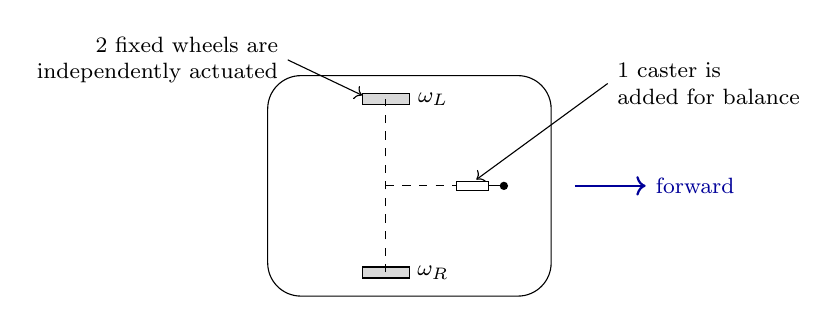
\begin{tikzpicture}[font=\footnotesize]
\draw[rounded corners=12pt] (-1.8,-1.4) rectangle (1.8,1.4);
\fixedwheel{-0.3,1.1}{0}\fixedwheel{-0.3,-1.1}{0}
\draw[dashed] (-0.3,-1.1)--(-0.3,1.1);
\draw[dashed] (-0.3,0)--(1.2,0);
\casterwheel{1.2,0}{0}
\node at (0.3,1.1) {$\omega_L$}; \node at (0.3,-1.1) {$\omega_R$};
\draw[->,thick,blue!60!black] (2.1,0)--(3.0,0) node[right]{forward};
\node[align=right] (n1) at (-3.2,1.6) {2 fixed wheels are\\independently actuated};
\draw[->] (n1.east)--(-0.6,1.15);
\node[align=left] (n2) at (3.8,1.3) {1 caster is\\added for balance};
\draw[->] (n2.west)--(0.85,0.08);
\end{tikzpicture}
\caption{Differential-drive robot (slide 9), top view.}
\end{figure}

% \begin{proposition}[Preview of the kinematics \emph{(beyond the slides)}]
% Let $r$ be the wheel radius, $d$ the distance between the wheels, $\omega_L,\omega_R$ the wheel speeds. Then the chassis forward speed $v$ and angular speed $\omega$ are
% \[
% v=\frac{r}{2}(\omega_R+\omega_L),\qquad \omega=\frac{r}{d}(\omega_R-\omega_L).
% \]
% \end{proposition}
% \begin{proof}
% The contact points move at $v_R=r\omega_R$ and $v_L=r\omega_L$. By rigid-body kinematics $v_R=v+\omega d/2$ and $v_L=v-\omega d/2$; adding and subtracting these equations gives the claim.
% \end{proof}

\begin{intuition}
It is a tank (or a wheelchair): equal speeds drive straight, different speeds curve towards the slower wheel, opposite speeds spin on the spot. With $r=0.1$\,m, $d=0.4$\,m: $\omega_R=\omega_L=5$\,rad/s gives $v=0.5$\,m/s, $\omega=0$; $\omega_R=-\omega_L=5$\,rad/s gives $v=0$, $\omega=2.5$\,rad/s. The slides show an indoor mobile base and a robot vacuum cleaner as examples. The caster only keeps the robot from tipping, as the balance section requires.
\end{intuition}

\subsection{Synchro-drive mobile robot \emph{(slide 10)}}

\begin{definition}[Synchro-drive WMR]
A WMR with \textbf{3 orientable wheels} that are \textbf{simultaneously actuated}. The orientation of the chassis remains constant.
\end{definition}

\begin{figure}[H]
\centering
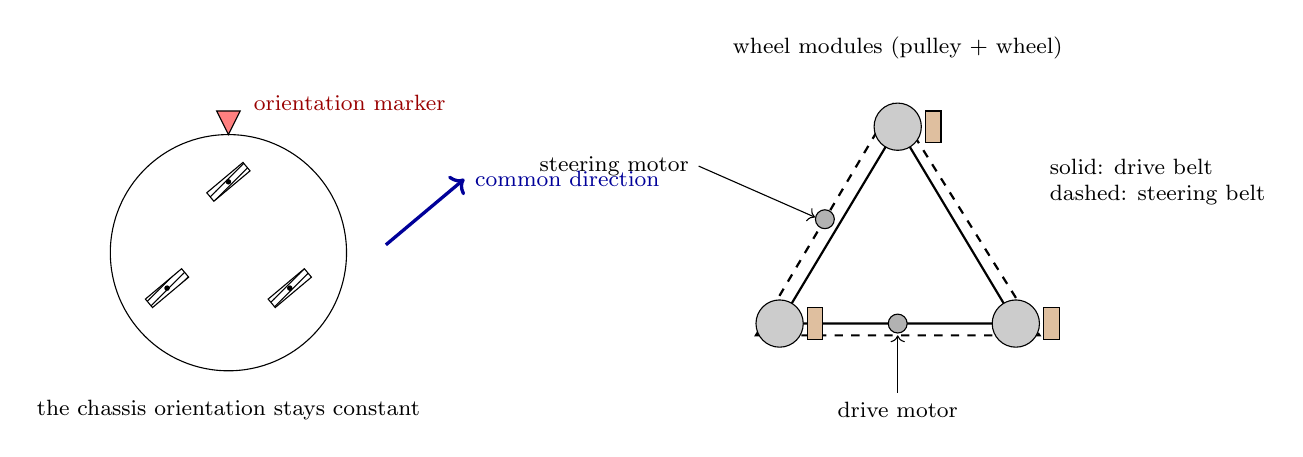
\begin{tikzpicture}[font=\footnotesize]
\draw (0,0) circle (1.5);
\orientwheel{90:0.9}{40}\orientwheel{210:0.9}{40}\orientwheel{330:0.9}{40}
\draw[fill=red!50] (0,1.5)--(-0.15,1.8)--(0.15,1.8)--cycle;
\node[red!60!black,right] at (0.2,1.9) {orientation marker};
\draw[->,very thick,blue!60!black] (2.0,0.1)--++(40:1.3) node[right]{common direction};
\node at (0,-2.0) {the chassis orientation stays constant};
% belt schematic
\begin{scope}[xshift=8.5cm]
\coordinate (T) at (0,1.6); \coordinate (L) at (-1.5,-0.9); \coordinate (R) at (1.5,-0.9);
\draw[thick] (T)--(L)--(R)--cycle;
\draw[dashed,thick] (-0.05,1.9)--(-1.8,-1.05)--(1.8,-1.05)--cycle;
\foreach \p in {T,L,R} { \draw[fill=gray!40] (\p) circle (0.3);
  \draw[fill=brown!50] ($(\p)+(0.35,-0.2)$) rectangle ($(\p)+(0.55,0.2)$); }
\draw[fill=gray!60] (0,-0.9) circle (0.12);
\draw[fill=gray!60] (-0.925,0.425) circle (0.12);
\node[align=left] at (3.3,0.9) {solid: drive belt\\dashed: steering belt};
\node[align=right] (m1) at (-3.6,1.1) {steering motor};
\draw[->] (m1.east)--(-1.05,0.45);
\node (m2) at (0,-2.0) {drive motor};
\draw[->] (m2.north)--(0,-1.05);
\node at (0,2.6) {wheel modules (pulley + wheel)};
\end{scope}
\end{tikzpicture}
\caption{Synchro-drive (slide 10). Left: three orientable wheels, always parallel. Right: simplified drive train redrawn from the slide: one drive motor and one steering motor act on all the wheels through belts.}
\end{figure}

% \begin{proposition}[Constant chassis orientation \emph{(beyond the slides)}]
% If all wheels have the same steering angle and the same rolling speed, the chassis undergoes a pure translation: its angular velocity is zero.
% \end{proposition}
% \begin{proof}
% With pure rolling, the contact point of each wheel moves along the wheel plane with speed $r\omega_{\text{wheel}}$. Since the planes are parallel and the speeds equal, all contact points have the \emph{same} velocity vector. For two distinct points $A,B$ of a rigid body $v_B-v_A=\omega\times(B-A)=0$, which forces $\omega=0$.
% \end{proof}

\begin{intuition}
The three wheels are like three people pushing a table in exactly the same direction at the same speed: the table translates and never turns. The robot changes its direction of travel by turning all wheels together, but its body keeps pointing the same way; that is why the sensors or the ``head'' of a synchro-drive robot would need their own rotation mechanism (the slide shows a laptop riding on top). The price of this simplicity is a drive train with belts, but only two motors for three wheels.
\end{intuition}

\subsection{Tricycle and car-like robots \emph{(slide 11)}}

\begin{definition}[Tricycle]
\textbf{2 fixed wheels} on a common axle and \textbf{1 orientable wheel}.
\end{definition}
\begin{definition}[Car-like]
\textbf{2 fixed wheels} on a common axle and \textbf{2 orientable wheels} on a common axle.
\end{definition}
Both may be front-wheel drive or rear-wheel drive.

\begin{figure}[H]
\centering
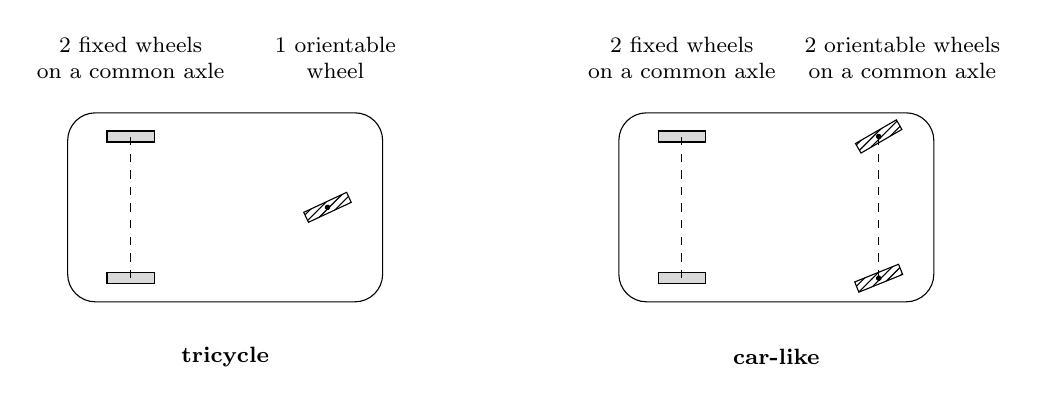
\begin{tikzpicture}[font=\footnotesize]
% tricycle
\draw[rounded corners=10pt] (-1.8,-1.2) rectangle (2.2,1.2);
\fixedwheel{-1,0.9}{0}\fixedwheel{-1,-0.9}{0}
\draw[dashed] (-1,-0.9)--(-1,0.9);
\orientwheel{1.5,0}{25}
\node at (0.2,-1.9) {\textbf{tricycle}};
\node[align=center] at (-1.0,1.9) {2 fixed wheels\\on a common axle};
\node[align=center] at (1.6,1.9) {1 orientable\\wheel};
% car-like
\begin{scope}[xshift=7cm]
\draw[rounded corners=10pt] (-1.8,-1.2) rectangle (2.2,1.2);
\fixedwheel{-1,0.9}{0}\fixedwheel{-1,-0.9}{0}
\draw[dashed] (-1,-0.9)--(-1,0.9);
\orientwheel{1.5,0.9}{30}\orientwheel{1.5,-0.9}{22}
\draw[dashed] (1.5,-0.9)--(1.5,0.9);
\node at (0.2,-1.9) {\textbf{car-like}};
\node[align=center] at (-1.0,1.9) {2 fixed wheels\\on a common axle};
\node[align=center] at (1.8,1.9) {2 orientable wheels\\on a common axle};
\end{scope}
\end{tikzpicture}
\caption{Tricycle (left) and car-like robot (right), top views (slide 11). The tilted wheels are steered.}
\end{figure}

% \begin{proposition}[Ackermann steering \emph{(beyond the slides)}]
% Let $\ell$ be the wheelbase and $w$ the distance between the steerable wheels. If the steering axes (perpendicular to each wheel plane) of a car-like robot meet in a single point of the rear-axle line, the inner and outer steering angles $\delta_i,\delta_o$ satisfy
% \[
% \cot\delta_o-\cot\delta_i=\frac{w}{\ell}.
% \]
% \end{proposition}
% \begin{proof}
% Let $R$ be the distance from the centre of rotation to the middle of the rear axle. Then $\tan\delta_i=\ell/(R-w/2)$ and $\tan\delta_o=\ell/(R+w/2)$. Taking reciprocals and subtracting gives $w/\ell$.
% \end{proof}

\begin{intuition}
When a car turns, each wheel must roll along a circle with the same centre, and the inner circle is smaller; the inner wheel therefore has to turn more than the outer one. Numbers: $\ell=2.5$\,m, $w=1.5$\,m, $\delta_i=30^\circ$: $\cot\delta_o=1.732+0.6=2.332$, so $\delta_o\approx23.2^\circ$. A tricycle, with only one steered wheel, does not have this issue. Front-wheel drive means the steered wheel(s) are also driven; rear-wheel drive means the fixed axle is driven, which requires the device of the next subsection when the two rear wheels share a motor.
\end{intuition}

\subsection{The differential \emph{(slide 12)}}

\begin{definition}[Differential]
A mechanical device needed whenever two \emph{driving} wheels are mounted on a \emph{common axle} (driven by the same motor), which allows the two wheels to move at \emph{different speeds}.
\end{definition}

\begin{figure}[H]
\centering
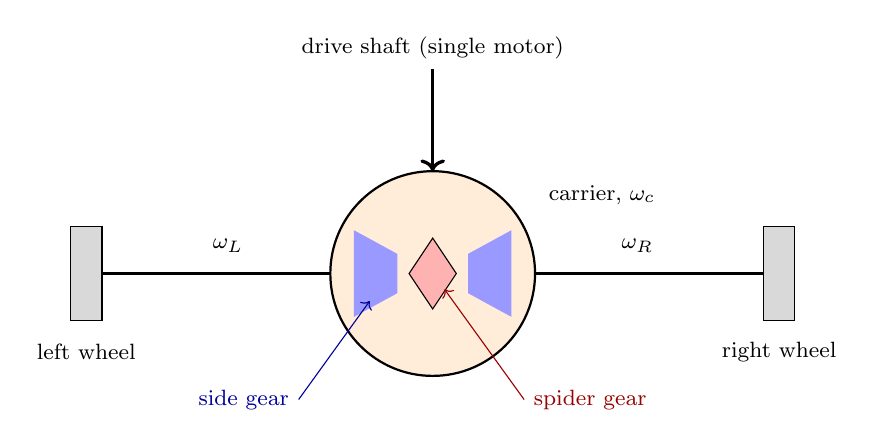
\begin{tikzpicture}[font=\footnotesize]
\draw[fill=gray!30] (-4.6,-0.6) rectangle (-4.2,0.6);
\draw[fill=gray!30] (4.2,-0.6) rectangle (4.6,0.6);
\draw[very thick] (-4.2,0)--(-1.0,0); \draw[very thick] (1.0,0)--(4.2,0);
\draw[thick,fill=orange!15] (0,0) circle (1.3);
\fill[blue!40] (-1.0,-0.55)--(-1.0,0.55)--(-0.45,0.25)--(-0.45,-0.25)--cycle;
\fill[blue!40] (1.0,-0.55)--(1.0,0.55)--(0.45,0.25)--(0.45,-0.25)--cycle;
\draw[fill=red!30] (0,0.45)--(0.3,0)--(0,-0.45)--(-0.3,0)--cycle;
\draw[very thick,->] (0,2.6)--(0,1.3);
\node[above] at (0,2.6) {drive shaft (single motor)};
\node at (-4.4,-1.0) {left wheel}; \node at (4.4,-1.0) {right wheel};
\node at (-2.6,0.35) {$\omega_L$}; \node at (2.6,0.35) {$\omega_R$};
\node[right] at (1.35,1.0) {carrier, $\omega_c$};
\node[blue!60!black] (sg) at (-2.4,-1.6) {side gear}; \draw[->,blue!60!black] (sg.east)--(-0.8,-0.35);
\node[red!60!black] (sp) at (2.0,-1.6) {spider gear}; \draw[->,red!60!black] (sp.west)--(0.15,-0.2);
\end{tikzpicture}
\caption{Schematic of a differential (idealised). The slide shows an animated 3D model.}
\end{figure}

% \begin{proposition}[Ideal open differential \emph{(beyond the slides)}]
% For an ideal differential the carrier (the part driven by the motor) rotates at the average of the two wheel speeds,
% \[
% \omega_c=\frac{\omega_L+\omega_R}{2},
% \]
% and the motor torque $\tau$ is split equally: $\tau_L=\tau_R=\tau/2$.
% \end{proposition}
% \begin{proof}
% Seen from the carrier, the spider gear reverses the rotation, so the two side gears turn at equal and opposite relative speeds: $\omega_L-\omega_c=-(\omega_R-\omega_c)$. Solving gives $\omega_c=(\omega_L+\omega_R)/2$. The spider gear is a lever with two equal arms in equilibrium, so it transmits equal forces to the two side gears.
% \end{proof}

\begin{intuition}
Why is it needed? When a car turns, the outer wheel travels along a longer arc than the inner one, so the two must rotate at different speeds; if rigidly tied to one shaft they would drag and slip. The differential lets the wheels share the motor while spinning differently. Numbers: wheels at 4 and 6\,rad/s $\Rightarrow$ the carrier turns at 5\,rad/s. A known side effect of equal torque split: if one wheel is on ice, it can only transmit a tiny torque, and so can the other.
\end{intuition}

\subsection{Firetruck \emph{(slide 13)}}

\begin{definition}[Firetruck]
A \textbf{tractor} (car-like) coupled to a \textbf{trailer} having \textbf{2 orientable wheels on a common axle}.
\end{definition}

\begin{figure}[H]
\centering
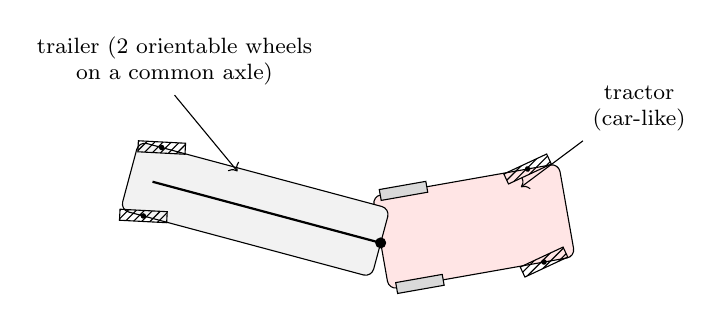
\begin{tikzpicture}[font=\footnotesize]
\coordinate (T) at (3.2,0.5);
\coordinate (H) at ($(T)+(190:1.2)$);
\begin{scope}[shift={(T)},rotate=10]
\draw[rounded corners=3pt,fill=red!10] (-1.2,-0.6) rectangle (1.2,0.6);
\fixedwheel{-0.8,0.6}{0}\fixedwheel{-0.8,-0.6}{0}
\orientwheel{0.8,0.6}{15}\orientwheel{0.8,-0.6}{15}
\end{scope}
\begin{scope}[shift={(H)},rotate=-15]
\draw[rounded corners=3pt,fill=gray!10] (-3.3,-0.45) rectangle (0,0.45);
\orientwheel{-3.0,0.45}{12}\orientwheel{-3.0,-0.45}{12}
\draw[thick] (0,0)--(-3.0,0);
\end{scope}
\fill (H) circle (2pt);
\node[align=center] (a) at (5.3,2.0) {tractor\\(car-like)};
\draw[->] (a.south west)--(3.8,1.0);
\node[align=center] (b) at (-0.6,2.6) {trailer (2 orientable wheels\\on a common axle)};
\draw[->] (b.south)--(0.2,1.2);
\end{tikzpicture}
\caption{Firetruck (slide 13), top view; the dot is the hitch.}
\end{figure}

\begin{intuition}
A ladder firetruck is very long. A second person (the ``tiller operator'', as the slide's overlay says) steers the \emph{rear} axle so that the trailer does not cut the corner and can pass around cars and curbs. In kinematic terms, it is a car-like robot pulling a trailer with its own steering.
\end{intuition}

\subsection{Omnidirectional robots with actuated caster wheels \emph{(slide 14)}}

\begin{definition}[Omnidirectional WMR]
A WMR that can instantaneously move in any direction of the plane, \emph{without first re-orienting the chassis}, and rotate independently of translation.)
\end{definition}

The structure on the slide uses \textbf{active caster wheels}, i.e.\ caster wheels that are both steered and driven.

\begin{figure}[H]
\centering
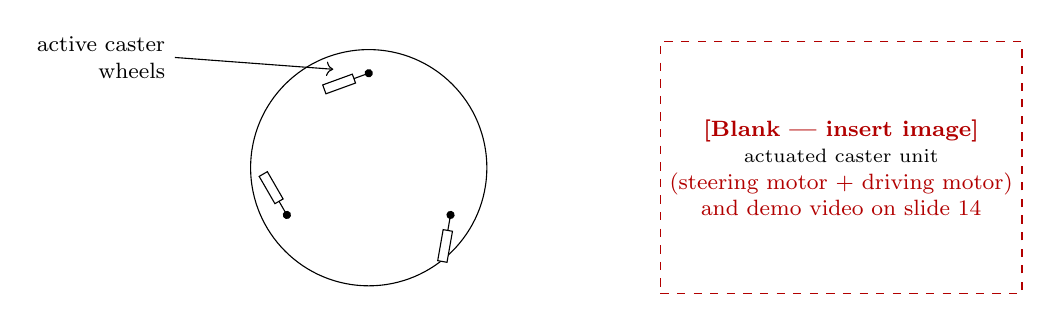
\begin{tikzpicture}[font=\footnotesize]
\draw (0,0) circle (1.5);
\casterwheel{90:1.2}{20}\casterwheel{210:1.2}{-60}\casterwheel{330:1.2}{80}
\node[align=right] (c) at (-3.4,1.4) {active caster\\wheels};
\draw[->] (c.east)--(-0.45,1.25);
\node[draw=red!70!black,dashed,minimum width=4.2cm,minimum height=3.2cm,align=center,text=red!70!black] at (6.0,0) {\textbf{[Blank --- insert image]}\\\scriptsize\color{black}actuated caster unit\\(steering motor + driving motor)\\and demo video on slide 14};
\end{tikzpicture}
\caption{Omnidirectional robot with three active casters (slide 14, left drawing) and a spot for the slide's photo/video.}
\end{figure}

\begin{intuition}
Each wheel can point wherever it likes and be driven at the right speed, so it can follow the velocity that its own mount point must have. If all wheels point the same way, the robot translates in that direction; if their directions differ, the robot rotates. The effect is like a shopping cart that can instantly go sideways.So something that a car can't do, however the cost is mechanical: two motors per wheel. So more expensive, more complex and also more difficult to control than a differential-drive robot, but it can move in any direction without turning first.
\end{intuition}

\subsection{Mecanum (Swedish) wheels \emph{(slide 15)}}

\begin{definition}[Mecanum wheel]
A wheel with a ring of free-spinning rollers mounted around its rim, with the roller axes oblique to the wheel axle. Omnidirectional mobile robots can be built using Mecanum (Swedish) wheels.
\end{definition}

\begin{figure}[H]
\centering
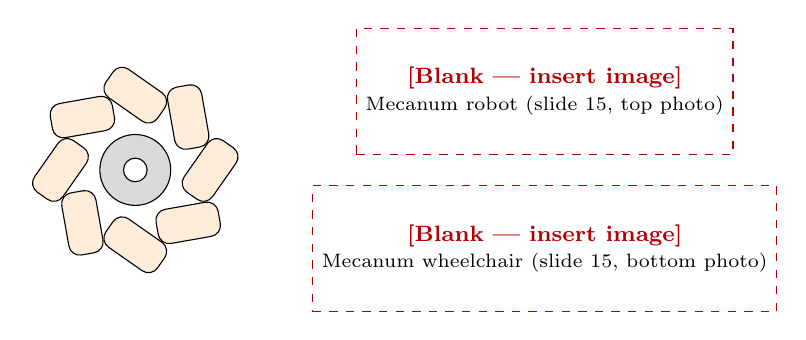
\begin{tikzpicture}[font=\footnotesize]
\foreach \a in {0,45,...,315}{
  \begin{scope}[shift={(\a:0.95)},rotate=\a+55]
  \draw[rounded corners=4pt,fill=orange!15] (-0.4,-0.22) rectangle (0.4,0.22);
  \end{scope}}
\draw[fill=gray!30] (0,0) circle (0.45);
\draw[fill=white] (0,0) circle (0.15);
\node[draw=red!70!black,dashed,minimum width=3.6cm,minimum height=1.6cm,align=center,text=red!70!black] at (5.2,1.0) {\textbf{[Blank --- insert image]}\\\scriptsize\color{black}Mecanum robot (slide 15, top photo)};
\node[draw=red!70!black,dashed,minimum width=3.6cm,minimum height=1.6cm,align=center,text=red!70!black] at (5.2,-1.0) {\textbf{[Blank --- insert image]}\\\scriptsize\color{black}Mecanum wheelchair (slide 15, bottom photo)};
\end{tikzpicture}
\caption{A Mecanum wheel seen along its axle (slide 15, left drawing) and spots for the two photos.}
\end{figure}

\begin{intuition}
The rollers turn the ``wheel'' into one that can roll forward \emph{and} slide sideways freely: the ground force of each wheel acts along the axis of its roller instead of along the wheel plane. Choosing the speeds of several such wheels, one can obtain any combination of forward, sideways and rotational motion of the chassis, with no steering mechanism at all, a purely fixed-axle structure that is nonetheless omnidirectional.The problem is that the rollers have to be really close to the ground to transmit force, so the robot has to be very low to the ground. The slide shows a small robot and a wheelchair as examples.
\end{intuition}

% =====================================================================
\part{Wheels: Constraints and Mobility}
 
\section{Wheels (constraints \& mobility) \emph{(page 1)}}
 
Wheels do not merely support the robot: they \emph{introduce constraints} on its motion. We can study them in four steps:
\begin{itemize}[nosep]
  \item \textbf{geometric constraints} (GC), which limit the configurations $q$ the robot can take;
  \item \textbf{kinematic constraints} (KC), which limit the velocities $\dot q$ it can have;
  \item the \textbf{relationships} between GC and KC;
  \item the resulting \textbf{mobility} of the robot,
\end{itemize}
and then apply everything to the example of \textbf{rolling wheels}.
 
\begin{intuition}
Compare a bead on a wire with an ice skater. The bead can never leave the wire: a restriction on \emph{where} it can be. The skater's blade cannot slide sideways at any instant: a restriction on \emph{how} she can move, yet she can still reach every point of the rink. Both are ``constraints'' but of two different natures, and this part of the lecture is about telling them apart. Wheels turn out to be of the skater type.
\end{intuition}
 
% ---------------------------------------------------------------------
\section{Geometric constraints (GC) \emph{(pages 1--2)}}
 
\subsection{Constraints on the configuration \emph{(page 1)}}
 
\begin{definition}[Configuration space]
The configuration of the robot is a vector $q\in\mathcal C$ of generalized coordinates, where the configuration space $\mathcal C$ is (locally) $\simeq\mathbb R^n$. The number $n$ is the number of coordinates.
\end{definition}
 
Constraints are classified along two axes: \emph{equality} (bilateral) vs.\ \emph{inequality} (unilateral), and \emph{time-variant} vs.\ \emph{time-invariant}.
 
\begin{table}[H]
\centering\small
\begin{tabular}{@{}lll@{}}
\toprule
 & time-invariant & time-variant\\
\midrule
equality (bilateral) & $h(q)=0$ & $h(q,t)=0$\\
inequality (unilateral) & $h(q)\ge 0$ & $h(q,t)\ge 0$\\
\bottomrule
\end{tabular}
\caption{Classification of constraints on $q$ (page 1). Only the first column of the first row is studied here.}
\end{table}
 
\begin{definition}[Geometric constraint]
Among the equality, time-invariant constraints, a \emph{geometric constraint} (GC) has the form
\[
h_i(q)=0,\qquad i=1,\dots,k,
\]
and \emph{depends only on $q$}.
\end{definition}
 
\begin{figure}[H]
\centering
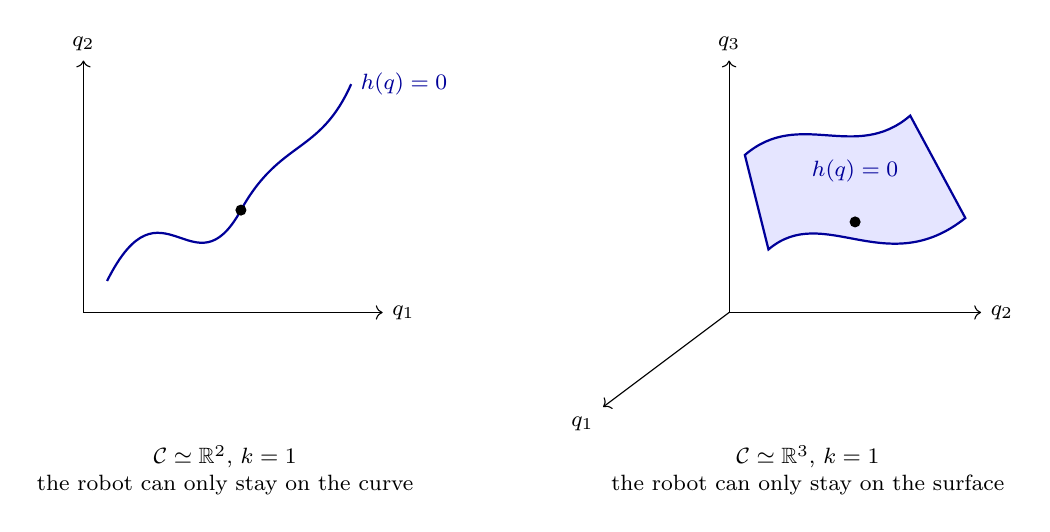
\begin{tikzpicture}[font=\footnotesize]
\draw[->] (0,0)--(3.8,0) node[right]{$q_1$};
\draw[->] (0,0)--(0,3.2) node[above]{$q_2$};
\draw[thick,blue!60!black] (0.3,0.4) .. controls (1.0,1.8) and (1.4,0.2) .. (2.0,1.3) .. controls (2.5,2.2) and (3.0,2.0) .. (3.4,2.9);
\node[blue!60!black,right] at (3.4,2.9) {$h(q)=0$};
\fill (2.0,1.3) circle (2pt);
\node[align=center] at (1.8,-2.0) {$\mathcal C\simeq\mathbb R^2$, $k=1$\\the robot can only stay on the curve};
\begin{scope}[xshift=8.2cm]
\draw[->] (0,0)--(3.2,0) node[right]{$q_2$};
\draw[->] (0,0)--(0,3.2) node[above]{$q_3$};
\draw[->] (0,0)--(-1.6,-1.2) node[below left]{$q_1$};
\draw[thick,blue!60!black,fill=blue!10] (0.5,0.8) .. controls (1.2,1.4) and (2.0,0.4) .. (3.0,1.2) -- (2.3,2.5) .. controls (1.6,1.9) and (0.9,2.6) .. (0.2,2.0) -- cycle;
\node[blue!60!black] at (1.6,1.8) {$h(q)=0$};
\fill (1.6,1.15) circle (2pt);
\node[align=center] at (1.0,-2.0) {$\mathcal C\simeq\mathbb R^3$, $k=1$\\the robot can only stay on the surface};
\end{scope}
\end{tikzpicture}
\caption{Geometric constraints (page 1): the dot is the robot, which must remain on the curve (left) or surface (right) $h(q)=0$.}
\end{figure}
 
\begin{intuition}
A bead threaded on a wire has $n=2$ coordinates in the plane but one constraint ($k=1$): it lives on a curve. A point constrained to a surface in space ($n=3$, $k=1$) lives on a surface. In general, $k$ constraints leave an $(n-k)$-dimensional world for the robot to live in.
\end{intuition}
 
\subsection{Mobility limitation and reduced coordinates \emph{(page 2)}}
 
\begin{proposition}[Global mobility limitation]\label{prop:global}
If the constraints $h_1(q)=\dots=h_k(q)=0$ are independent, i.e.\ $\partial h/\partial q$ has rank $k$, the set $\{q: h(q)=0\}$ is (locally) an $(n-k)$-dimensional subset of $\mathcal C$, and the robot configuration must remain in it for all times.
\end{proposition}
\begin{proof}
This is the implicit function theorem (regular value theorem): around any solution, $k$ coordinates can be expressed as smooth functions of the remaining $n-k$.
\end{proof}
 
We call this a \emph{global} mobility limitation: wherever the robot is, it is confined to a lower-dimensional subset.
 
\begin{intuition}
Are we then ``wasting'' the $k$ remaining coordinates? Yes: they are determined by the other $n-k$. The number $n-k$ is the \emph{number of degrees of freedom} (DOF), and one may try to describe the robot with a ``reduced'' configuration vector of $n-k$ coordinates: solve the GC for $k$ coordinates as functions of the independent ones and keep only the latter.
\end{intuition}
 
\begin{example}[The circle]\label{ex:circle}
Take $q=(q_1,q_2)\in\mathbb R^2$ with $q_1^2+q_2^2=1$. Solving for $q_2$ gives $q_2=\pm\sqrt{1-q_1^2}$. This is only a \emph{local} resolution: it needs a choice of branch, and at $q_1=\pm1$ the derivative $\partial h/\partial q_2=2q_2$ vanishes, so the square root breaks down (a \emph{singularity}). So \emph{we don't do that}. We use different coordinates instead, here the arc length $s\in[0,2\pi)$, with $q=(\cos s,\sin s)$.
\end{example}
 
\begin{figure}[H]
\centering
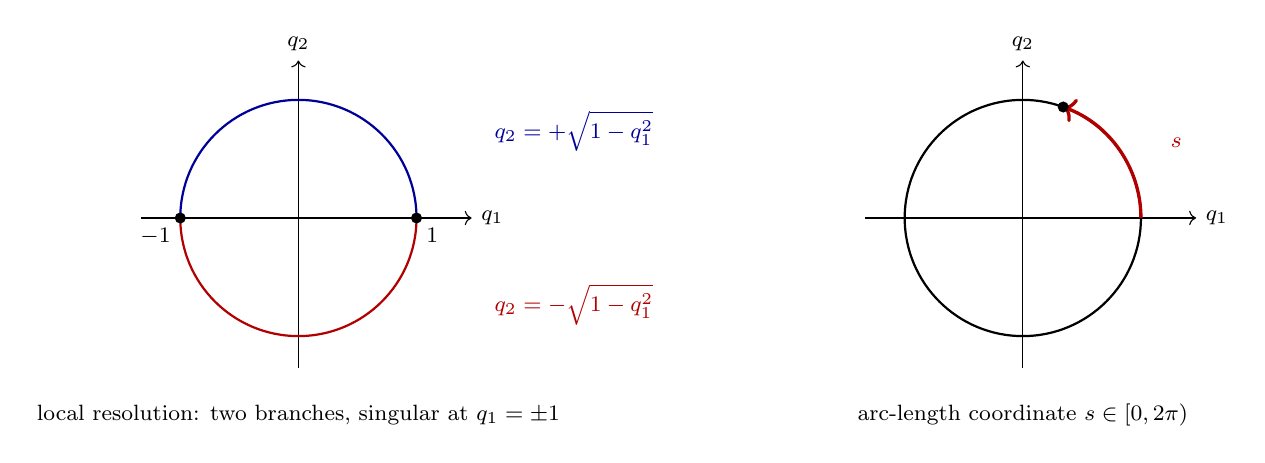
\begin{tikzpicture}[font=\footnotesize]
\draw[->] (-2,0)--(2.2,0) node[right]{$q_1$};
\draw[->] (0,-1.9)--(0,2.0) node[above]{$q_2$};
\draw[thick,blue!60!black] (1.5,0) arc (0:180:1.5);
\draw[thick,red!70!black] (-1.5,0) arc (180:360:1.5);
\fill (1.5,0) circle (2pt); \fill (-1.5,0) circle (2pt);
\node[below right] at (1.5,0) {$1$}; \node[below left] at (-1.5,0) {$-1$};
\node[blue!60!black,align=left] at (3.5,1.1) {$q_2=+\sqrt{1-q_1^2}$};
\node[red!70!black,align=left] at (3.5,-1.1) {$q_2=-\sqrt{1-q_1^2}$};
\node at (0,-2.5) {local resolution: two branches,\ singular at $q_1=\pm1$};
\begin{scope}[xshift=9.2cm]
\draw[->] (-2,0)--(2.2,0) node[right]{$q_1$};
\draw[->] (0,-1.9)--(0,2.0) node[above]{$q_2$};
\draw[thick] (0,0) circle (1.5);
\draw[->,very thick,red!70!black] (1.5,0) arc (0:70:1.5);
\fill (70:1.5) circle (2pt);
\node[red!70!black] at (1.95,0.95) {$s$};
\node at (0,-2.5) {arc-length coordinate $s\in[0,2\pi)$};
\end{scope}
\end{tikzpicture}
\caption{The circle $q_1^2+q_2^2=1$ (page 2): solving the GC for one coordinate versus using a single new coordinate $s$.}
\end{figure}
 
\begin{intuition}
It is the difference between describing a point on the Earth's equator by ``the latitude as a square root of something'' and simply by its \emph{longitude}: the longitude (our arc length $s$) is one honest coordinate that wraps around, with no branches and no singular points. In general one picks new coordinates that automatically satisfy the GC, instead of solving the constraint equations.
\end{intuition}
 
% ---------------------------------------------------------------------
\section{Kinematic constraints (KC) \emph{(page 3)}}
 
\begin{definition}[Kinematic constraint]
A \emph{kinematic constraint} (KC) has the form
\[
a_i(q,\dot q)=0,\qquad i=1,\dots,k,
\]
where $\dot q$ are the \emph{generalized velocities} (time derivatives). It depends on $q$ \emph{and} $\dot q$; at any $q$ it is a constraint on $\dot q$.
\end{definition}
 
\begin{definition}[Pfaffian form]
A KC is in \emph{Pfaffian form} when $\dot q$ appears \emph{linearly}:
\[
a_i^{T}(q)\,\dot q=0,\quad i=1,\dots,k
\qquad\Longleftrightarrow\qquad
A(q)\,\dot q=0,\quad A(q)=\begin{bmatrix}a_1^{T}(q)\\ \vdots\\ a_k^{T}(q)\end{bmatrix}.
\]
KC are typically found in this form.
\end{definition}
 
\begin{proposition}[Admissible velocities]
At each configuration $q$ the admissible generalized velocities are exactly those in the null space $\mathcal N(A(q))$. If $A(q)$ has rank $k$, this is a linear subspace of dimension $n-k$.
\end{proposition}
\begin{proof}
$A(q)\dot q=0$ is the definition of the null space, whose dimension is $n-\operatorname{rank}A(q)=n-k$ by rank--nullity.
\end{proof}
 
\begin{example}
For $n=3$ and the single constraint $a^{T}=(2,\,-1,\,0)$, i.e.\ $2\dot q_1-\dot q_2=0$, the admissible velocities are $\dot q=\alpha(1,2,0)^{T}+\beta(0,0,1)^{T}$: a plane ($n-k=2$ dimensions) in velocity space.
\end{example}
 
\begin{intuition}
The KC does not forbid any \emph{place}; it forbids some \emph{ways of moving} at each place: at every $q$ the allowed velocities form a plane (or subspace), and the plane can change with $q$. This is a \textbf{local} mobility limitation. The number of instantaneous degrees of freedom is still $n-k$, but \emph{we cannot ``reduce'' the configuration vector}: all $n$ coordinates are still needed (whether this is really so is the subject of the next section).
\end{intuition}
 
% ---------------------------------------------------------------------
\section{Relationships between GC and KC \emph{(pages 4--6)}}
 
\subsection{Any GC implies a KC \emph{(pages 4--5)}}
 
\begin{proposition}[GC $\Rightarrow$ KC]\label{prop:gckc}
Every GC $h(q)=0$ implies the Pfaffian KC
\[
\dot h(q)=\frac{\partial h}{\partial q}\,\dot q=\bigl(\nabla_q h\bigr)^{T}\dot q=0 ,
\]
i.e.\ $a^{T}(q)=\partial h/\partial q$. Hence admissible velocities belong to the tangent plane of the surface $h(q)=0$ at every $q$.
\end{proposition}
\begin{proof}
For the constraint to hold as time goes by, it must hold continuously: $h(q(t))\equiv0$, so $\dot h=0$. Since $q$ depends on time, the chain rule gives $\frac{\partial h}{\partial q}\dot q=0$, where $\bigl(\frac{\partial h}{\partial q_1},\dots,\frac{\partial h}{\partial q_n}\bigr)=(\nabla_q h)^{T}$ is the gradient. This is a KC in Pfaffian form.
\end{proof}
 
\begin{figure}[H]
\centering
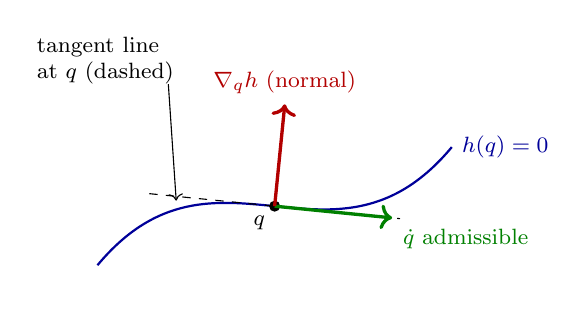
\begin{tikzpicture}[font=\footnotesize]
\draw[thick,blue!60!black] (0,0) .. controls (1.5,1.8) and (3,-0.3) .. (4.5,1.5) node[right]{$h(q)=0$};
\fill (2.25,0.75) circle (2pt); \node[below left] at (2.25,0.75) {$q$};
\draw[dashed] (2.25,0.75)++(174.3:1.6) -- ++(-5.7:3.2);
\draw[->,very thick,green!50!black] (2.25,0.75)--++(-5.7:1.5) node[below right]{$\dot q$ admissible};
\draw[->,very thick,red!70!black] (2.25,0.75)--++(84.3:1.3) node[above]{$\nabla_q h$ (normal)};
\node[align=left] at (0.1,2.6) {tangent line\\at $q$ (dashed)};
\draw[->] (0.9,2.3)--(1.0,0.82);
\end{tikzpicture}
\caption{The gradient $\nabla_q h$ is normal to the surface $h(q)=0$; admissible velocities are tangent to it, so $(\nabla_q h)^{T}\dot q=0$ (page 4).}
\end{figure}
 
\begin{intuition}
Imagine hiking on a hillside: your velocity must be tangent to the slope, never pointing into the ground or up into the air. The gradient is the arrow sticking out of the surface (the normal), and ``$a^{T}\dot q=0$'' simply says that the velocity is \emph{orthogonal to the normal}: a dot product between orthogonal vectors is zero. So every geometric constraint secretly hides a velocity constraint.
\end{intuition}
 
\subsection{The converse: integrable vs.\ non-integrable \emph{(pages 5--6)}}
 
Can we say the contrary, i.e.\ that a KC $a^{T}(q)\dot q=0$ implies a GC $h(q)=0$? In general no, sometimes yes: it depends on whether the KC can be \emph{integrated}.
 
\begin{definition}[Holonomic / nonholonomic]
A Pfaffian KC $a^{T}(q)\dot q=0$ is \emph{integrable} (\emph{holonomic}) if there exist a function $h(q)$ and a function $\gamma(q)\neq0$ such that
\[
\frac{\partial h}{\partial q}=\gamma(q)\,a^{T}(q),
\]
so that the KC is equivalent to $\dot h=0$, i.e.\ to the GC $h(q)=\text{const}$. Otherwise it is \emph{non-integrable} (\emph{nonholonomic}), which is the general case.
\end{definition}
 
\begin{example}[Integrable: circles]\label{ex:circles}
In $\mathbb R^2$, $q=(q_1,q_2)^{T}$, take $q_1\dot q_1+q_2\dot q_2=0$, i.e.\ $a^{T}(q)=(q_1,\ q_2)$. Consider $q_1^2+q_2^2=C$ and differentiate: $2q_1\dot q_1+2q_2\dot q_2=0$; dividing by 2 gives the KC. So it is \emph{integrable}, with $h=q_1^2+q_2^2$ ($\gamma=2$) and $C$ an integration constant.
\end{example}
 
\begin{proposition}[Local limitation $\Rightarrow$ global limitation]\label{prop:l2g}
If a KC is integrable, every admissible trajectory stays on a level set of $h$: $h(q(t))=h(q(0))$ for all $t$.
\end{proposition}
\begin{proof}
$\frac{d}{dt}h(q(t))=\frac{\partial h}{\partial q}\dot q=\gamma(q)\,a^{T}(q)\dot q=0$.
\end{proof}
 
\begin{example}[Left open by the professor: $q_2\dot q_1+q_1\dot q_2=0$ \emph{(solution by me, not in the notes)}]
Here $a^{T}=(q_2,\ q_1)$ and $h(q)=q_1q_2$ satisfies $\partial h/\partial q=(q_2,q_1)=a^{T}$ (with $\gamma=1$): the KC is integrable and the robot is confined to a hyperbola $q_1q_2=c$.
\end{example}
 
\begin{figure}[H]
\centering
\begin{tikzpicture}[font=\footnotesize]
\foreach \r in {0.6,1.1,1.6} \draw[dashed,gray] (0,0) circle (\r);
\draw[thick,blue!60!black] (0,0) circle (1.1);
\draw[->] (-2.0,0)--(2.2,0) node[right]{$q_1$};
\draw[->] (0,-1.9)--(0,2.0) node[above]{$q_2$};
\fill (130:1.1) circle (2pt);
\draw[->,very thick,green!50!black] (130:1.1)--++(220:0.8);
\draw[->,very thick,green!50!black] (130:1.1)--++(40:0.8);
\draw[->,thick] (0,0)--(-25:1.1) node[midway,below]{$\sqrt C$};
\node at (0,-2.6) {$q_1^2+q_2^2=C$};
\begin{scope}[xshift=7.2cm]
\draw[->] (-2.8,0)--(2.9,0) node[right]{$q_1$};
\draw[->] (0,-2.8)--(0,2.9) node[above]{$q_2$};
\draw[thick,blue!60!black] plot[domain=0.2:2.5,samples=30] (\x,{0.5/\x});
\draw[thick,blue!60!black] plot[domain=0.55:2.7,samples=30] (\x,{1.5/\x});
\draw[thick,blue!60!black] plot[domain=0.2:2.5,samples=30] (-\x,{-0.5/\x});
\draw[thick,blue!60!black] plot[domain=0.55:2.7,samples=30] (-\x,{-1.5/\x});
\node[blue!60!black] at (2.0,1.4) {$q_1q_2=c$};
\node at (0,-3.4) {$q_1q_2=c$};
\end{scope}
\end{tikzpicture}
\caption{Left: the KC $q_1\dot q_1+q_2\dot q_2=0$ is tangent to circles: starting at a point we cannot leave the circle (page 6). Right: the KC $q_2\dot q_1+q_1\dot q_2=0$ integrates to hyperbolas.}
\end{figure}
 
\begin{intuition}
At each point the admissible velocity is tangent to a curve; chaining these tiny tangent steps, you simply trace the curve out: you can never hop onto another circle. This is why we can say: \emph{the local limitation (of the KC) implies a global limitation (of the GC)}. The function $\gamma$ is just a rescaling: multiplying the constraint by a non-zero factor does not change which velocities are admissible. How does one know if a constraint is integrable without guessing $h$? There are mathematical tools, such as \textbf{Frobenius' theorem}.
\end{intuition}
 
\begin{theorem}[Frobenius, single constraint in $\mathbb R^3$ \emph{(stated without proof)}]\label{thm:frob}
Let $a(q)\neq0$, $q\in\mathbb R^3$. The constraint $a^{T}(q)\dot q=0$ is integrable if and only if $a\cdot(\nabla\times a)=0$.
\end{theorem}
 
% ---------------------------------------------------------------------
\section{Example: rolling wheels \emph{(pages 7--9)}}
 
\subsection{The rolling disk and the pure rolling constraint \emph{(page 7)}}
 
If the KC is \textbf{not integrable} (nonholonomic), the mobility limitation is \emph{purely local}. The key example is the rolling disk.
 
\begin{definition}[Rolling disk]
A disk (wheel) that stays upright while rolling on the plane. Its configuration is $q=(x,y,\theta)^{T}$, where $(x,y)$ is the contact point and $\theta$ the orientation of the wheel plane (heading).
\end{definition}
 
\begin{lemma}[Pure rolling constraint]
Pure rolling without lateral slip means that the instantaneous velocity of the contact point has no component along the unit normal $n=(\sin\theta,\,-\cos\theta)^{T}$ to the wheel plane:
\[
\sin\theta\,\dot x-\cos\theta\,\dot y=0,
\quad\text{i.e.}\quad
\underbrace{(\sin\theta,\ -\cos\theta)}_{n^{T}}\begin{pmatrix}\dot x\\ \dot y\end{pmatrix}=0 .
\]
In the full configuration space this is the Pfaffian KC
\[
a^{T}(q)\,\dot q=(\sin\theta,\ -\cos\theta,\ 0)\begin{pmatrix}\dot x\\ \dot y\\ \dot\theta\end{pmatrix}=0 .
\]
\end{lemma}
\begin{proof}
A velocity $(\dot x,\dot y)$ orthogonal to $n$ is parallel to the heading $(\cos\theta,\sin\theta)$; the formula is the orthogonality condition $n^{T}(\dot x,\dot y)^{T}=0$, with a zero entry for $\dot\theta$ since the constraint does not involve it.
\end{proof}
 
\begin{figure}[H]
\centering
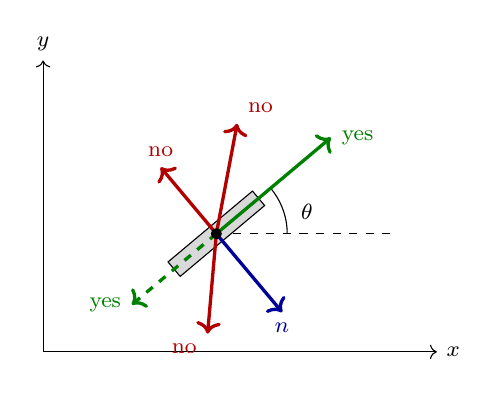
\begin{tikzpicture}[font=\footnotesize]
\draw[->] (0,0)--(5.0,0) node[right]{$x$};
\draw[->] (0,0)--(0,3.7) node[above]{$y$};
\draw[dashed] (2.2,1.5)--(4.4,1.5);
\draw (3.1,1.5) arc (0:40:0.9); \node at (3.35,1.78) {$\theta$};
\begin{scope}[shift={(2.2,1.5)},rotate=40]
\draw[fill=gray!30] (-0.7,-0.12) rectangle (0.7,0.12);
\draw[->,very thick,green!50!black] (0,0)--(1.9,0) node[right]{yes};
\draw[->,very thick,green!50!black,dashed] (0,0)--(-1.4,0) node[left]{yes};
\draw[->,very thick,red!70!black] (0,0)--(1.1,0.9) node[above right]{no};
\draw[->,very thick,red!70!black] (0,0)--(0,1.1) node[above]{no};
\draw[->,very thick,red!70!black] (0,0)--(-0.9,-0.9) node[below left]{no};
\draw[->,very thick,blue!60!black] (0,0)--(0,-1.3) node[below]{$n$};
\end{scope}
\fill (2.2,1.5) circle (2pt);
\end{tikzpicture}
\caption{Top view of the rolling disk (page 7); the dot is the contact point $(x,y)$. Velocities of the contact point with a component along the normal $n$ are forbidden (``no''); only motion along the wheel plane is allowed (``yes'').}
\end{figure}
 
\begin{intuition}
It is the ice-skater's blade: the contact point can glide forwards or backwards along the blade, but can never slide sideways, so the velocity is always lined up with $\theta$. Since the condition concerns \emph{instantaneous} velocity, it is a \emph{local} mobility constraint. In fact the null space of $a^{T}(q)$ is spanned by $g_1=(\cos\theta,\sin\theta,0)^{T}$ (roll) and $g_2=(0,0,1)^{T}$ (spin): $\dot q=g_1v+g_2\omega$, with $n-k=3-1=2$ admissible directions at each configuration.
\end{intuition}
 
\subsection{Is pure rolling integrable? \emph{(page 8)}}
 
\begin{proposition}[Pure rolling is non-integrable]\label{prop:frobroll}
The pure rolling constraint is non-integrable.
\end{proposition}

 
We decide to avoid the use of Frobenius' theorem and prove it \emph{constructively}, by proposing a maneuver that moves the disk from anywhere to everywhere: the \emph{universal maneuver}.
 
\begin{algorithm}[Universal maneuver]\label{alg:universal}
Input: start $q_s=(x_s,y_s,\theta_s)$ and goal $q_g=(x_g,y_g,\theta_g)$, with $(x_g,y_g)\neq(x_s,y_s)$. Let $\varphi=\operatorname{atan2}(y_g-y_s,\,x_g-x_s)$.
\begin{enumerate}[nosep]
  \item \textbf{Pure rotation} about the vertical axis, $\dot x=\dot y=0$, from $\theta_s$ to $\varphi$ (the KC is satisfied).
  \item \textbf{Pure rolling}, $\dot q=v(\cos\varphi,\sin\varphi,0)^{T}$, until $(x_g,y_g)$ is reached (the KC is satisfied because the contact point velocity is always aligned with $\theta=\varphi$).
  \item \textbf{Pure rotation} from $\varphi$ to $\theta_g$ (the KC is satisfied).
\end{enumerate}
(If $(x_g,y_g)=(x_s,y_s)$, only a rotation is needed.)
\end{algorithm}
 
\begin{figure}[H]
\centering
\begin{tikzpicture}[font=\footnotesize]
\draw[->] (-0.6,-0.4)--(6.4,-0.4) node[right]{$x$};
\draw[->] (-0.6,-0.4)--(-0.6,3.7) node[above]{$y$};
\fixedwheel{0.5,0.5}{-30}
\ghostwheel{0.5,0.5}{24}
\ghostwheel{5,2.5}{24}
\fixedwheel{5,2.5}{100}
\draw[->] ($(0.5,0.5)+(-30:0.6)$) arc (-30:24:0.6);
\draw[->] ($(5,2.5)+(24:0.6)$) arc (24:100:0.6);
\draw[->,very thick,blue!60!black] ($(0.5,0.5)+(24:0.7)$) -- ($(5,2.5)-(24:0.7)$);
\node[draw,circle,inner sep=1pt] at (0.9,1.25) {1};
\node[draw,circle,inner sep=1pt] at (2.5,1.95) {2};
\node[draw,circle,inner sep=1pt] at (5.6,3.3) {3};
\node[below] at (0.5,0.1) {$q_s$};
\node[right] at (5.55,2.0) {$q_g$};
\end{tikzpicture}
\caption{The universal maneuver (page 8): \textcircled{1} rotate in place towards the goal, \textcircled{2} roll straight to $(x_g,y_g)$, \textcircled{3} rotate to the final orientation. Dashed: intermediate configurations.}
\end{figure}
 
\begin{proposition}[The maneuver is universal]\label{alg:universal}
For any $q_s,q_g\in\mathbb R^2\times S^1$, Algorithm~\ref{alg:universal} produces a path that satisfies the pure rolling constraint at every instant and connects $q_s$ to $q_g$.
\end{proposition}
\begin{proof}
During phases 1 and 3, $\dot x=\dot y=0$ so $a^{T}\dot q=0\cdot\sin\theta-0\cdot\cos\theta+0\cdot\dot\theta=0$. During phase 2, $\theta=\varphi$ is constant and $\dot q=v(\cos\varphi,\sin\varphi,0)$, so $a^{T}\dot q=v(\sin\varphi\cos\varphi-\cos\varphi\sin\varphi)=0$. The three phases end respectively at heading $\varphi$, at position $(x_g,y_g)$ and at heading $\theta_g$.
\end{proof}
 
\begin{corollary}[Non-integrability]
The pure rolling constraint is non-holonomic.
\end{corollary}
\begin{proof}
If it were integrable, by Proposition~\ref{prop:l2g} every admissible trajectory would stay on a level set of a function $h$ with $\partial h/\partial q=\gamma a^{T}\neq0$, so $h$ would not be constant; but by the universal maneuver~\ref{alg:universal} admissible paths connect any two configurations, so $h$ would be constant on $\mathbb R^2\times S^1$. Contradiction.
\end{proof}
 
\begin{example}
Let $q_s=(0,0,0)$ and $q_g=(1,1,\pi/2)$ (metres, radians). Then $\varphi=\pi/4$: rotate by $\pi/4$ in place, roll $\sqrt2\approx1.41$\,m along the diagonal, then rotate by another $\pi/4$ to reach $\theta_g=\pi/2$.
\end{example}
 
\begin{intuition}
It is the recipe of ``turn towards the goal, walk straight, turn to the final direction''. Each of the three motions is allowed by the KC, and together they reach \emph{any} configuration, even though at every instant only 2 of the 3 directions of $q$-space are admissible. A constraint that could be integrated would trap the robot on a curve or surface, whereas here nothing traps it.
\end{intuition}
 
\subsection{No global mobility limitation \emph{(page 9)}}
 
Hence there is \textbf{no global mobility limitation}: the KC \emph{must be non-holonomic}. Here we illustrate this with a ``naive representation'' of $\mathcal C$ and with parallel parking.
 
\begin{example}[Parallel parking of a rolling disk]
Let $q_s=(0,0,0)$ and $q_g=(0,2,0)$: the goal is 2\,m to the side, with the same orientation. The direct motion $\dot y\neq0$ with $\theta=0$ is not admissible, since $a^{T}\dot q=-\dot y\neq0$: parallel parking \emph{cannot be done instantaneously}. It can be done with three admissible moves: (1) rotate to $\theta=\pi/2$; (2) roll 2\,m along $y$ (at $\theta=\pi/2$ the constraint reads $\dot x=0$, so $y$ is free); (3) rotate back to $\theta=0$.
\end{example}
 
\begin{figure}[H]
\centering
\begin{minipage}[b]{0.48\linewidth}
\centering
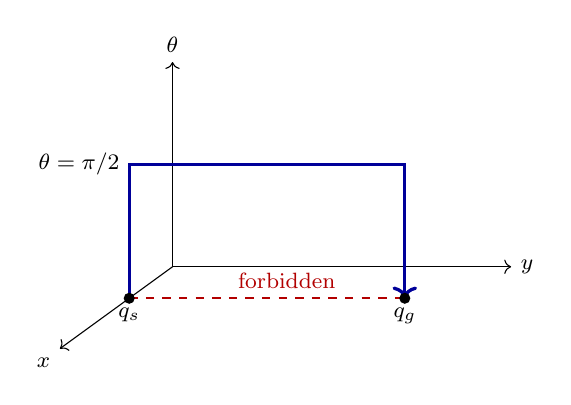
\begin{tikzpicture}[font=\footnotesize,x={(-0.55cm,-0.4cm)},y={(1cm,0cm)},z={(0cm,1cm)}]
\draw[->] (0,0,0)--(2.6,0,0) node[below left]{$x$};
\draw[->] (0,0,0)--(0,4.3,0) node[right]{$y$};
\draw[->] (0,0,0)--(0,0,2.6) node[above]{$\theta$};
\draw[red!70!black,dashed,thick] (1,0,0)--(1,3.5,0);
\draw[->,very thick,blue!60!black] (1,0,0)--(1,0,1.7)--(1,3.5,1.7)--(1,3.5,0);
\fill (1,0,0) circle (2pt); \fill (1,3.5,0) circle (2pt);
\node[below] at (1,0,0) {$q_s$}; \node[below] at (1,3.5,0) {$q_g$};
\node[left] at (1,0,1.7) {$\theta=\pi/2$};
\node[red!70!black,above] at (1,2.0,0) {forbidden};
\end{tikzpicture}
\\[2pt]\small (a) path in $\mathcal C$
\end{minipage}\hfill
\begin{minipage}[b]{0.48\linewidth}
\centering
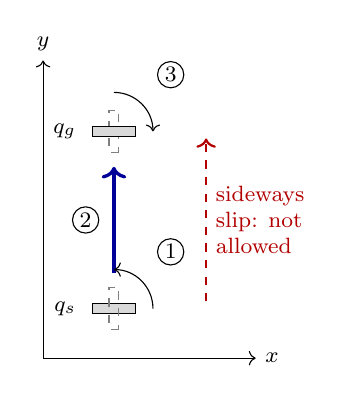
\begin{tikzpicture}[font=\footnotesize,scale=0.9]
\draw[->] (-1.0,-0.7)--(2.0,-0.7) node[right]{$x$};
\draw[->] (-1.0,-0.7)--(-1.0,3.5) node[above]{$y$};
\fixedwheel{0,0}{0}
\ghostwheel{0,0}{90}
\ghostwheel{0,2.5}{90}
\fixedwheel{0,2.5}{0}
\draw[->,very thick,blue!60!black] (0,0.5)--(0,2.0);
\draw[->] (0.55,0) arc (0:90:0.55);
\draw[->] (0,3.05) arc (90:0:0.55);
\node[draw,circle,inner sep=1pt] at (0.8,0.8) {1};
\node[draw,circle,inner sep=1pt] at (-0.4,1.25) {2};
\node[draw,circle,inner sep=1pt] at (0.8,3.3) {3};
\node[left] at (-0.4,0) {$q_s$}; \node[left] at (-0.4,2.5) {$q_g$};
\draw[->,red!70!black,dashed,thick] (1.3,0.1)--(1.3,2.4);
\node[red!70!black,right,align=left] at (1.3,1.25) {sideways\\slip: not\\allowed};
\end{tikzpicture}
\\[2pt]\small (b) top view
\end{minipage}
\caption{Parallel parking (page 9). (a) In $\mathcal C=\mathbb R^2\times S^1$ the direct path at $\theta=0$ is forbidden; the admissible path climbs along the $\theta$ axis, moves along $y$, and comes back down. (b) The same maneuver seen from above.}
\end{figure}
 
\begin{intuition}
Think of the three coordinates $(x,y,\theta)$ as a 3D world in which the disk may move only along two of the three directions at each point; yet by combining the motions, like a sailor tacking against the wind, every point becomes reachable. So the kinematic constraint \emph{reduces how you can move} (local), but \emph{not where you can get to} (global). Compare the two kinds of constraint: an integrable KC is a GC in disguise (global limitation, the dimension of the reachable set drops to $n-k$); a non-integrable KC (rolling) keeps all $n$ coordinates alive and limits only the instantaneous velocities.
\end{intuition}
 
% =====================================================================
\section{Summary}
 
\subsection{Part I: kinematic structures of WMRs}
 
\begin{table}[H]
\centering\footnotesize
\renewcommand{\arraystretch}{1.25}
\begin{tabular}{@{}>{\raggedright\arraybackslash}p{2.4cm}>{\raggedright\arraybackslash}p{3.9cm}>{\raggedright\arraybackslash}p{4.9cm}>{\raggedright\arraybackslash}p{2.5cm}@{}}
\toprule
Structure & Wheels & Key feature & Slide examples\\
\midrule
Differential-drive & 2 fixed, independently actuated, + 1 caster (balance) & Steering through the speed difference of the two wheels & indoor base, robot vacuum cleaner\\
Synchro-drive & 3 orientable, simultaneously actuated & Wheels always parallel; chassis orientation constant & cylindrical robot with laptop\\
Tricycle & 2 fixed on a common axle + 1 orientable & Front- or rear-wheel drive & ---\\
Car-like & 2 fixed + 2 orientable, each pair on a common axle & Front- or rear-wheel drive; differential for a driven common axle & ---\\
Firetruck & car-like tractor + trailer with 2 orientable wheels on a common axle & Trailer steered separately by the tiller operator & ladder truck\\
Omni, active casters & active caster wheels (steered and driven) & Any direction without re-orienting; 2 motors per wheel & actuated caster unit\\
Omni, Mecanum & wheels with oblique free rollers & Omnidirectional with fixed wheel axles & small robot, wheelchair\\
\bottomrule
\end{tabular}
\caption{Part I: comparison of the WMR kinematic structures (slides 9--15).}
\end{table}
 
\begin{figure}[H]
\centering
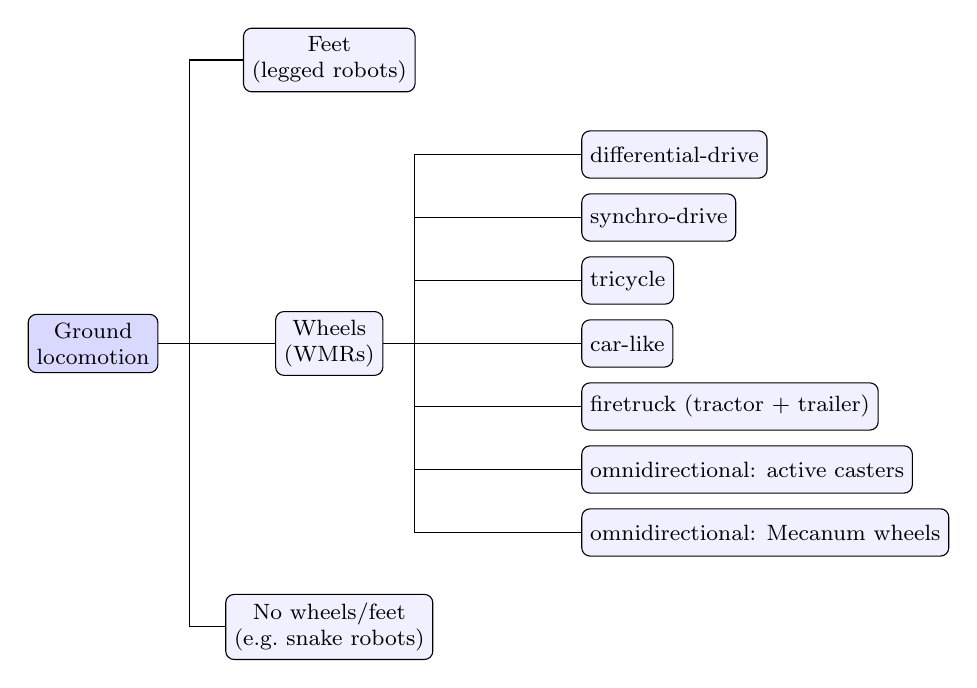
\begin{tikzpicture}[font=\footnotesize,
  box/.style={draw,rounded corners=3pt,fill=blue!6,minimum height=0.6cm,align=center,inner sep=3pt}]
\node[box,fill=blue!15] (root) at (0,0) {Ground\\locomotion};
\node[box] (w) at (3.0,0) {Wheels\\(WMRs)};
\node[box] (l) at (3.0,3.6) {Feet\\(legged robots)};
\node[box] (o) at (3.0,-3.6) {No wheels/feet\\(e.g.\ snake robots)};
\node[box,anchor=west] (n1) at (6.2,2.4) {differential-drive};
\node[box,anchor=west] (n2) at (6.2,1.6) {synchro-drive};
\node[box,anchor=west] (n3) at (6.2,0.8) {tricycle};
\node[box,anchor=west] (n4) at (6.2,0) {car-like};
\node[box,anchor=west] (n5) at (6.2,-0.8) {firetruck (tractor + trailer)};
\node[box,anchor=west] (n6) at (6.2,-1.6) {omnidirectional: active casters};
\node[box,anchor=west] (n7) at (6.2,-2.4) {omnidirectional: Mecanum wheels};
\foreach \n in {w,l,o} \draw (root.east)--++(0.4,0) |- (\n.west);
\foreach \n in {n1,n2,n3,n4,n5,n6,n7} \draw (w.east)--++(0.4,0) |- (\n.west);
\end{tikzpicture}
\caption{Part I map: from ground locomotion to the WMR kinematic structures.}
\end{figure}
 
\subsection{Part II: constraints and mobility}
 
\begin{table}[H]
\centering\footnotesize
\renewcommand{\arraystretch}{1.25}
\begin{tabular}{@{}>{\raggedright\arraybackslash}p{2.9cm}>{\raggedright\arraybackslash}p{3.1cm}>{\raggedright\arraybackslash}p{4.4cm}>{\raggedright\arraybackslash}p{3.2cm}@{}}
\toprule
Constraint & Form & Mobility limitation & Example\\
\midrule
Geometric (GC) & $h(q)=0$, depends only on $q$ & \emph{Global}: $q$ confined to an $(n-k)$-dimensional set; reduced coordinates possible & circle $q_1^2+q_2^2=1$, arc length $s$\\
Kinematic, integrable (holonomic) & $a^{T}(q)\dot q=0$ with $\partial h/\partial q=\gamma\,a^{T}$ & Equivalent to a GC: local limitation implies a global one & $q_1\dot q_1+q_2\dot q_2=0$: circles\\
Kinematic, non-integrable (nonholonomic) & $a^{T}(q)\dot q=0$, no such $h$ & \emph{Purely local}: $\dot q\in\mathcal N(A(q))$; every configuration is reachable; $q$ cannot be reduced & rolling disk $\sin\theta\,\dot x-\cos\theta\,\dot y=0$\\
\bottomrule
\end{tabular}
\caption{Part II: types of constraints and their effect on mobility (pages 1--9).}
\end{table}
 
\begin{figure}[H]
\centering
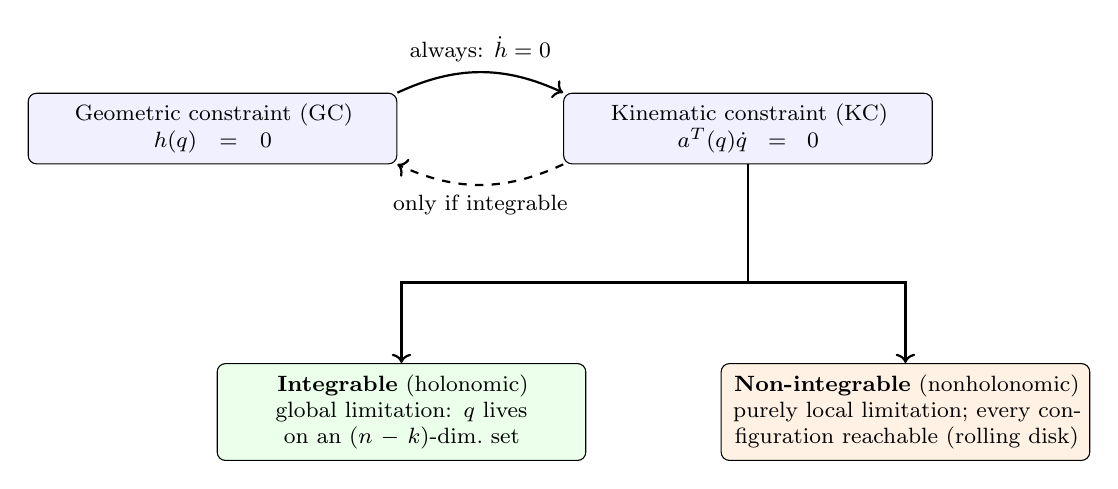
\begin{tikzpicture}[font=\footnotesize,
  box/.style={draw,rounded corners=3pt,fill=blue!6,align=center,text width=4.4cm,inner sep=4pt}]
\node[box] (A) at (0,0) {Geometric constraint (GC)\\$h(q)=0$};
\node[box] (B) at (6.8,0) {Kinematic constraint (KC)\\$a^{T}(q)\dot q=0$};
\node[box,fill=green!8] (C) at (2.4,-3.6) {\textbf{Integrable} (holonomic)\\global limitation: $q$ lives on an $(n-k)$-dim.\ set};
\node[box,fill=orange!10] (D) at (8.8,-3.6) {\textbf{Non-integrable} (nonholonomic)\\purely local limitation; every configuration reachable (rolling disk)};
\draw[->,thick] (A.north east) to[bend left=25] node[above]{always: $\dot h=0$} (B.north west);
\draw[->,thick,dashed] (B.south west) to[bend left=25] node[below]{only if integrable} (A.south east);
\draw[->,thick] (B.south) -- ++(0,-1.5) -| (C.north);
\draw[->,thick] (B.south) -- ++(0,-1.5) -| (D.north);
\end{tikzpicture}
\caption{Part II map: relationships between geometric and kinematic constraints.}
\end{figure}
 
\subsection{Key take-aways}
\begin{itemize}
  \item Ground locomotion needs contact (wheels or feet). Static balance requires the CoM projection inside the support polygon, hence at least 3 wheels; dynamic balance replaces the CoM with the ZMP.
  \item Wheels come in three types (fixed, orientable, caster) which combine into the classical structures: differential-drive, synchro-drive, tricycle, car-like, tractor--trailer, and omnidirectional robots (active casters or Mecanum wheels); a differential is needed when two driven wheels share an axle.
  \item Wheels introduce constraints on $q$. A geometric constraint $h(q)=0$ confines the robot globally to an $(n-k)$-dimensional set; a kinematic constraint $a^{T}(q)\dot q=0$ restricts the velocities locally to the null space of $A(q)$.
  \item Every GC implies a KC (the velocity must be tangent to the surface, $\dot h=0$); the converse holds only for integrable (holonomic) KC, for which the local limitation implies a global one.
  \item Pure rolling, $\sin\theta\,\dot x-\cos\theta\,\dot y=0$, is non-integrable (Frobenius, or the universal ``turn, roll, turn'' maneuver): there is no global mobility limitation, all of $(x,y,\theta)$ is reachable, but not instantaneously, as in parallel parking.
\end{itemize}

\newpage

% ======================================================================
% Lecture 3
% ======================================================================
\part{Lecture 3}

% =====================================================================
\section{Kinematic constraints and admissible motions}\emph{(page 1)}
% =====================================================================

Let the robot have a configuration vector $q\in\mathcal{C}\simeq\R^n$, where $n$ is the number of generalized coordinates. The wheels impose \emph{kinematic constraints} (KCs) that are linear in the generalized velocities.

\begin{definition}[Kinematic constraints]
A set of $k$ kinematic constraints is written in Pfaffian form
\[
A(q)\,\dq = 0, \qquad A(q)\in\R^{k\times n},
\]
where $k$ is the number of constraints and $n$ the number of generalized coordinates.
\end{definition}

\begin{definition}[Admissible motions]
A generalized velocity $\dq$ is \emph{admissible} at $q$ if $\dq\in\N(A(q))$, the null space of $A(q)$. If the constraints are independent, $\dim\N(A(q))=n-k=:m$.
\end{definition}

\begin{intuition}
The constraints do not forbid places, they forbid \emph{instantaneous directions of motion}. At each configuration $q$ the robot may move only along the directions in the null space. Think of a skate on ice: from any position it may glide along its blade, but not sideways. The set of allowed directions changes with the configuration, which is why $A$ depends on $q$.
\end{intuition}

Pick a basis $\{g_1(q),\dots,g_m(q)\}$ of $\N(A(q))$. Each $g_i:\mathcal{C}\to\R^n$ is a \emph{vector field}, and every admissible velocity is a combination
\[
\dq=\sum_{i=1}^{m} g_i(q)\,u_i = \begin{pmatrix} g_1(q) & \cdots & g_m(q)\end{pmatrix}\begin{pmatrix}u_1\\ \vdots\\ u_m\end{pmatrix},
\]
where the $u_i$ are scalar coefficients, i.e.\ the \emph{admissible velocities} (also called pseudo-velocities).

\begin{figure}[h]
\centering
\begin{tikzpicture}[>=Stealth,scale=1]
\draw[->] (0,0)--(6.2,0) node[right]{$q_1$};
\draw[->] (0,0)--(0,3.8) node[above]{$q_2$};
\fill (1.5,1) circle(1.6pt) node[below left]{$q$};
\draw[->,thick,blue!70!black] (1.5,1)--(2.8,1.7) node[above right]{$g_1(q)$};
\draw[->,thick,red!70!black] (1.5,1)--(2.4,0.15) node[below right]{$g_2(q)$};
\fill (4.2,2.4) circle(1.6pt) node[below left]{$q'$};
\draw[->,thick,blue!70!black] (4.2,2.4)--(5.0,3.4) node[above]{$g_1(q')$};
\draw[->,thick,red!70!black] (4.2,2.4)--(5.5,2.5) node[right]{$g_2(q')$};
\end{tikzpicture}
\caption{The basis vectors $g_i(q)$ are vector fields: at each configuration they give (generally different) admissible directions.}
\end{figure}

% =====================================================================
\section{Explicit representation: the kinematic model}\emph{(pages 2--3)}
% =====================================================================

\begin{definition}[Kinematic model]\label{def:km}
The \emph{kinematic model} (KM) of a robot with $m$ independent admissible directions is
\[
\dq=\sum_{i=1}^{m} g_i(q)\,u_i = G(q)\,u,\qquad G(q)\in\R^{n\times m}\ \text{(a tall matrix)},\ u\in\R^m .
\]
For a chosen input $u$, at each $q$ it returns the instantaneous motion $\dq$ the robot executes.
\end{definition}

The KM is a \emph{dynamical system} with
\begin{itemize}[nosep]
\item state $q\in\mathcal{C}\simeq\R^n$ and input $u\in\R^m$;
\item \emph{nonlinear} dependence on the state $q$ (linear in the input $u$);
\item \emph{driftless}: $u=0\Rightarrow \dq=0$, i.e.\ with no input the robot stays where it is.
\end{itemize}

\begin{intuition}
``Driftless'' means there is no momentum in a kinematic model: stop commanding and the robot stops. (Momentum and forces appear only in the \emph{dynamic} model, which is a different level of description.) ``Tall matrix'' simply says that we have more coordinates ($n$) than inputs ($m$): fewer commands than degrees of freedom of the configuration, which is exactly what the constraints cause.
\end{intuition}

\begin{proposition}[The KM is not unique]\label{prop:nonuniq}
Let $\dq=G(q)u$ be a kinematic model and $T(q)\in\R^{m\times m}$ any smooth invertible matrix. Then $\dq=G(q)T(q)\,u'$ is another kinematic model of the same robot, and the two describe the same set of admissible velocities.
\end{proposition}
\begin{proof}
The columns of $G'=GT$ are linear combinations of the columns of $G$, hence lie in $\N(A(q))$; they are independent because $T$ is invertible, so they are $m$ independent vectors in an $m$-dimensional space, i.e.\ a basis. Conversely any admissible $\dq=Gu=GT(T^{-1}u)$ is generated by $u'=T^{-1}u$.
\end{proof}

\begin{intuition}
The basis $\{g_1,\dots,g_m\}$ can be chosen in infinitely many ways (rotate, rescale, mix the vector fields), so \emph{all these models are equivalent}. Some choices are nevertheless better because the inputs $u_i$ get a physical \emph{interpretation} (e.g.\ ``forward speed'' and ``turning speed''). We will see this with the unicycle.
\end{intuition}

\subsection{The unconstrained robot}\emph{(page 3)}

\begin{example}[KM of an unconstrained robot]
If there are no kinematic constraints ($k=0$) and no geometric constraints, then $m=n$, $A$ is absent and a natural basis of $\R^n$ is the canonical one:
\[
\dq=\begin{pmatrix}1\\0\\ \vdots\\0\end{pmatrix}u_1+\dots+\begin{pmatrix}0\\ \vdots\\0\\1\end{pmatrix}u_n = u .
\]
This is the case of, e.g., a free-flying robot. Every generalized velocity is directly commanded: the robot is \emph{fully actuated}.
\end{example}

\paragraph{Block schemes.} The unconstrained robot is a bank of $n$ simple integrators; a constrained robot places the matrix $G(q)$ between the pseudo-velocities $u$ and the integrators, with $q$ fed back to $G$.

\begin{figure}[h]
\centering
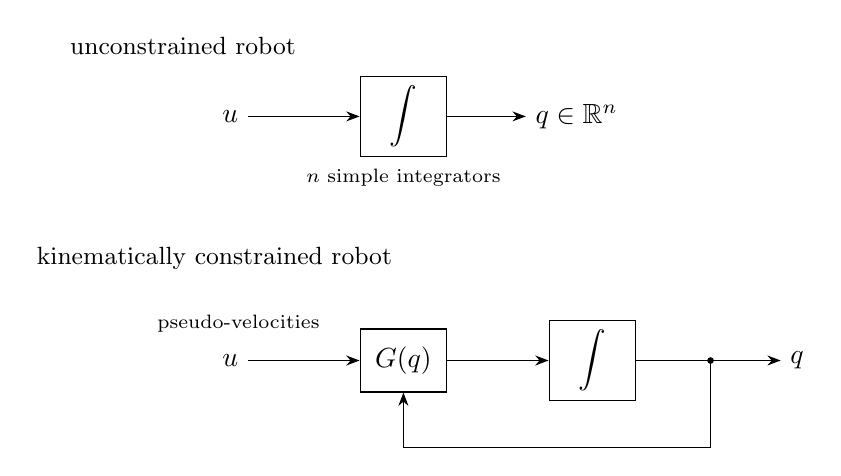
\begin{tikzpicture}[>=Stealth,box/.style={draw,minimum width=1.1cm,minimum height=0.8cm}]
% unconstrained
\node at (-0.6,0.9) {\small unconstrained robot};
\node (u1) at (0,0) {$u$};
\node[box] (I1) at (2.2,0) {$\displaystyle\int$};
\node (q1) at (4.4,0) {$q\in\R^n$};
\draw[->] (u1)--(I1);
\draw[->] (I1)--(q1);
\node[font=\scriptsize,below=1pt of I1] {$n$ simple integrators};
% constrained
\begin{scope}[yshift=-3.1cm]
\node at (-0.2,1.3) {\small kinematically constrained robot};
\node (u2) at (0,0) {$u$};
\node[box] (G) at (2.2,0) {$G(q)$};
\node[box] (I2) at (4.6,0) {$\displaystyle\int$};
\node (q2) at (7.2,0) {$q$};
\draw[->] (u2)--(G) node[midway,above,font=\scriptsize]{\strut};
\draw[->] (G)--(I2) node[midway,above]{$\dq$};
\draw[->] (I2)--(q2);
\fill (6.1,0) circle(1.2pt);
\draw[->] (6.1,0)--(6.1,-1.1)--(2.2,-1.1)--(G.south);
\node[font=\scriptsize,above=1pt of u2,xshift=3pt] {pseudo-velocities};
\end{scope}
\end{tikzpicture}
\caption{Block schemes of the kinematic model.}
\end{figure}

% =====================================================================
\section{Controllability of kinematic models}\emph{(page 4)}
% =====================================================================

\begin{definition}[Controllable KM]
A kinematic model is \emph{controllable} if for any initial configuration $q_i$ and any final configuration $q_f$ there exist a time $T$ and an input $u:[0,T]\to\R^m$ such that the solution of $\dq=G(q)u$ starting at $q_i$ reaches $q_f$ at time $T$.
\end{definition}

Controllability can be established in two ways: \emph{constructively}, by looking for a \emph{universal maneuver} that connects any pair of configurations, or by applying a \emph{test for controllability} (a rank condition, see Remark~\ref{rem:chow}).

\paragraph{Link with the constraints.} The notes relate controllability to the integrability of the kinematic constraints:
\begin{itemize}[nosep]
\item the KM is controllable $\iff$ the KCs are \emph{nonholonomic} (not integrable);
\item the KM is not controllable $\iff$ the KCs are \emph{holonomic}, i.e.\ integrable (partially or completely).
\end{itemize}

\begin{intuition}
If a constraint is integrable, it can be rewritten as a restriction on positions, $h(q)=\text{const}$ (for example $y=0$): the robot is trapped on a lower-dimensional surface and can never reach the other configurations, so the KM cannot be controllable. If the constraints are not integrable they leave the robot able to reach every configuration by sequencing admissible motions, as a car does when parallel parking: it cannot move sideways instantaneously, but it can reach any pose.
\end{intuition}

% =====================================================================
\section{The unicycle}\emph{(pages 4--6)}
% =====================================================================

\begin{definition}[Unicycle]
The unicycle is a vehicle with a single \emph{orientable} wheel. Its configuration is $q=(x,y,\theta)^{\!\top}$, where $(x,y)$ is the contact point and $\theta$ the orientation of the wheel's \emph{sagittal axis} with respect to the $x$-axis. The configuration space is $\mathcal{C}=\R^2\times \SO(2)$, locally $\simeq\R^3$ (hence $n=3$).
\end{definition}

\begin{figure}[h]
\centering
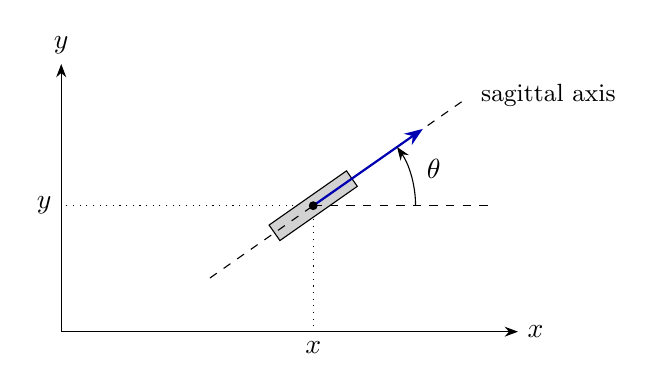
\begin{tikzpicture}[>=Stealth,scale=1]
\coordinate (P) at (3.2,1.6);
\draw[->] (0,0)--(5.8,0) node[right]{$x$};
\draw[->] (0,0)--(0,3.4) node[above]{$y$};
\draw[dotted] (P)--(3.2,0) node[below]{$x$};
\draw[dotted] (P)--(0,1.6) node[left]{$y$};
\begin{scope}[shift={(P)},rotate=35]
  \draw[fill=gray!35] (-0.6,-0.12) rectangle (0.6,0.12);
  \draw[dashed] (-1.6,0)--(2.4,0);
\end{scope}
\node[font=\small,anchor=west] at ($(P)+(35:2.45)$) {sagittal axis};
\draw[->,thick,blue!70!black] (P)--++(35:1.7) node[above]{};
\draw[dashed] (P)--++(2.3,0);
\draw[->] ($(P)+(1.3,0)$) arc (0:35:1.3);
\node at ($(P)+(17:1.6)$) {$\theta$};
\fill (P) circle(1.6pt);
\end{tikzpicture}
\caption{The unicycle seen from above: contact point $(x,y)$, sagittal axis at angle $\theta$.}
\end{figure}

\subsection{The pure rolling constraint}\emph{(page 5)}

The wheel rolls without slipping, so the contact point cannot move along the wheel axis (orthogonal to the sagittal axis):
\[
\sin\theta\,\dot x-\cos\theta\,\dot y=0 .
\]
Equivalently, $(\dot x,\dot y)$ must be \emph{aligned with the sagittal axis}, i.e.\ it has no component along the direction orthogonal to it. In Pfaffian form
\[
\underbrace{\begin{pmatrix}\sin\theta & -\cos\theta & 0\end{pmatrix}}_{A(q)}\begin{pmatrix}\dot x\\ \dot y\\ \dot\theta\end{pmatrix}=0,\qquad k=1,\ n=3,\ m=n-k=2 .
\]

\begin{intuition}
Worked numbers. At $\theta=0$: $A=(0,-1,0)$, so the constraint reads $\dot y=0$: the wheel may translate along $x$ and spin in place, never sideways. At $\theta=\pi/2$: $A=(1,0,0)$, so $\dot x=0$: now it may move along $y$ only. The forbidden direction rotates together with the wheel.
\end{intuition}

\begin{proposition}[Basis of the admissible velocities]\label{prop:basis}
A basis of $\N\big((\sin\theta\ \ {-\cos\theta}\ \ 0)\big)$, a 2-dimensional linear space, is
\[
g_1(q)=\begin{pmatrix}\cos\theta\\ \sin\theta\\ 0\end{pmatrix},\qquad g_2(q)=\begin{pmatrix}0\\0\\1\end{pmatrix}.
\]
\end{proposition}
\begin{proof}
$A g_1=\sin\theta\cos\theta-\cos\theta\sin\theta=0$ and $Ag_2=0$. The two vectors are linearly independent for every $\theta$, and $\dim\N(A)=3-1=2$.
\end{proof}

\paragraph{Kinematic model of the unicycle.}
\[
\dq=\begin{pmatrix}\cos\theta\\ \sin\theta\\ 0\end{pmatrix}u_1+\begin{pmatrix}0\\0\\1\end{pmatrix}u_2
\quad\Longleftrightarrow\quad
\begin{cases}\dot x=\cos\theta\,u_1\\ \dot y=\sin\theta\,u_1\\ \dot\theta=u_2 .\end{cases}
\]

\subsection{Interpretation of the inputs}\emph{(pages 5--6)}

From the model, $\dot x^2+\dot y^2=\cos^2\theta\,u_1^2+\sin^2\theta\,u_1^2=u_1^2$, hence
\[
u_1=\pm\sqrt{\dot x^2+\dot y^2}\quad(\text{equivalently }u_1=\cos\theta\,\dot x+\sin\theta\,\dot y),
\]
the magnitude of the velocity of the contact point, with sign $+$ for forward and $-$ for backward motion. We therefore rename
\[
u_1=v\ \text{(driving velocity)},\qquad u_2=\dot\theta=\omega\ \text{(steering velocity)} .
\]
The driving velocity is related to the angular velocity of the wheel about its own axis by $v=r\,\omega_{\rm roll}$ ($r$ = wheel radius, side view in Fig.~\ref{fig:wheel}); $\omega$ is the angular velocity of the wheel about the vertical axis.

\begin{definition}[Unicycle kinematic model]
\[
\dq=\begin{pmatrix}\cos\theta\\ \sin\theta\\ 0\end{pmatrix}v+\begin{pmatrix}0\\0\\1\end{pmatrix}\omega,
\qquad\text{i.e.}\quad
\begin{cases}\dot x=v\cos\theta\\ \dot y=v\sin\theta\\ \dot\theta=\omega .\end{cases}
\]
\end{definition}

\begin{figure}[h]
\centering
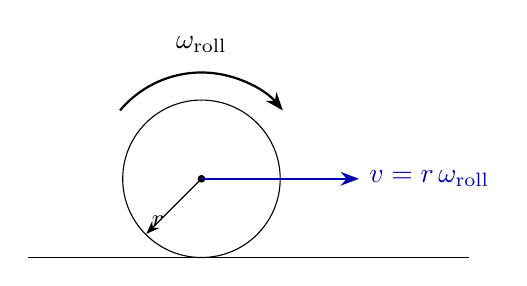
\begin{tikzpicture}[>=Stealth]
\draw (0,0) circle(1);
\fill (0,0) circle(1.4pt);
\draw[->] (0,0)--(-0.7,-0.7) node[midway,below left,font=\small]{$r$};
\draw[->,thick] (140:1.35) arc (140:40:1.35);
\node at (90:1.7) {$\omega_{\rm roll}$};
\draw (-2.2,-1)--(3.4,-1);
\draw[->,thick,blue!70!black] (0,0)--(2,0) node[right]{$v=r\,\omega_{\rm roll}$};
\end{tikzpicture}
\caption{Side view of the wheel: the driving velocity is $v=r\,\omega_{\rm roll}$.}\label{fig:wheel}
\end{figure}

\begin{intuition}
The basis $\{g_1,g_2\}$ was chosen so that the inputs are exactly what a driver feels: $v$ is ``how fast I roll along where I am pointing'' and $\omega$ is ``how fast I turn''. Any other basis (Proposition~\ref{prop:nonuniq}) would give an equivalent but less readable model. Constant inputs give circles: with $v=1\ \mathrm{m/s}$ and $\omega=0.5\ \mathrm{rad/s}$ the contact point moves on a circle of radius $v/\omega=2\ \mathrm m$ (see the figure in the Summary).
\end{intuition}

% =====================================================================
\section{Controllability of the unicycle}\emph{(page 7)}
% =====================================================================

\begin{proposition}\label{prop:unicycle-ctrl}
The unicycle KM is controllable: it can be steered from any $q_i=(x_i,y_i,\theta_i)$ to any $q_f=(x_f,y_f,\theta_f)$.
\end{proposition}

The notes answer ``yes'' by applying a universal maneuver, the same idea used earlier for the disk, in three steps.

\begin{algorithm}[Universal maneuver for the unicycle]\label{alg:maneuver}
Let $\varphi=\operatorname{atan2}(y_f-y_i,\ x_f-x_i)$ and $d=\sqrt{(x_f-x_i)^2+(y_f-y_i)^2}$.
\begin{enumerate}[nosep]
\item $v=0$, $\omega=$ constant, until $\theta=\varphi$ (rotate in place to point at the goal).
\item $v=$ constant, $\omega=0$, until $(x,y)=(x_f,y_f)$ (drive straight, distance $d$).
\item $v=0$, $\omega=$ constant, until $\theta=\theta_f$ (rotate in place to the final orientation).
\end{enumerate}
\end{algorithm}

\begin{proof}[Proof of Proposition~\ref{prop:unicycle-ctrl}]
During phases 1 and 3, $v=0$ gives $\dot x=\dot y=0$ and $\dot\theta=\omega$, so the position is frozen and $\theta$ changes at will; phase 1 takes $\theta$ from $\theta_i$ to $\varphi$ in time $T_1=(\varphi-\theta_i)/\omega$. During phase 2, $\omega=0$ keeps $\theta=\varphi$ constant, so $(\dot x,\dot y)=v(\cos\varphi,\sin\varphi)$ is a straight line, reaching $(x_f,y_f)$ after $T_2=d/v$. Phase 3 takes $\theta$ from $\varphi$ to $\theta_f$. (If $d=0$ phase 2 is skipped.)
\end{proof}

\begin{figure}[h]
\centering
\begin{tikzpicture}[>=Stealth,scale=1]
\coordinate (I) at (0,0);\coordinate (F) at (5.2,3);
\fill (I) circle(1.6pt) node[below left]{$q_i$};
\fill (F) circle(1.6pt) node[above right]{$q_f$};
\draw[->,thick] (I)--++(-20:1.0) node[right]{$\theta_i$};
\draw[dashed] (I)--(F);
\draw[->,very thick,blue!70!black] ($(I)+(-20:0.65)$) arc(-20:30:0.65);
\node[blue!70!black] at ($(I)+(5:0.95)$) {\small\textcircled{\scriptsize1}};
\draw[->,very thick,red!70!black] ($(I)!0.25!(F)$)--($(I)!0.75!(F)$);
\node[red!70!black,above left] at ($(I)!0.5!(F)$) {\small\textcircled{\scriptsize2}};
\draw[->,very thick,blue!70!black] ($(F)+(30:0.65)$) arc(30:100:0.65);
\node[blue!70!black] at ($(F)+(65:1.0)$) {\small\textcircled{\scriptsize3}};
\draw[->,thick] (F)--++(100:1.0) node[above]{$\theta_f$};
\end{tikzpicture}
\caption{Universal maneuver: rotate in place, drive straight, rotate in place.}
\end{figure}

\begin{intuition}
It is a ``point, drive, align'' strategy. Worked numbers: from $q_i=(0,0,0)$ to $q_f=(3,4,\pi/2)$ we have $\varphi=\arctan(4/3)\approx0.927$ rad ($53.1^\circ$) and $d=5$. With $|\omega|=1$ rad/s and $v=1$ m/s: rotate for $0.927$ s, drive for $5$ s, rotate for $\pi/2-0.927\approx0.644$ s ($36.9^\circ$). The two rotations ``cost'' nothing in position, which is possible only because the model lets us set $v=0$ and turn freely.
\end{intuition}

\begin{intuition}[Consistency with Section 3]
Despite the constraint $\dot y=0$ at $\theta=0$ (no sideways motion), the unicycle can reach any pose, because the pure rolling constraint is \emph{not integrable}: this is exactly the controllable/nonholonomic case.
\end{intuition}

\begin{lemma}[Rank test, supplementary]\label{rem:chow}
Let $[g_1,g_2]=\frac{\partial g_2}{\partial q}g_1-\frac{\partial g_1}{\partial q}g_2$ be the Lie bracket. For the unicycle $[g_1,g_2]=(\sin\theta,\,-\cos\theta,\,0)^{\!\top}$, and $\rank\{g_1,g_2,[g_1,g_2]\}=3=n$ for every $q$, so the controllability rank condition (Chow) holds.
\end{lemma}
\begin{proof}
$\partial g_2/\partial q=0$ and $\partial g_1/\partial q\,g_2=(-\sin\theta,\cos\theta,0)^{\!\top}$, hence $[g_1,g_2]=(\sin\theta,-\cos\theta,0)^{\!\top}$, which is orthogonal to $g_1$ and independent of $g_2$.
\end{proof}
\noindent\emph{(This is the ``test for controllability'' mentioned on page 4; the explicit computation is not in the handwritten notes.)}

\begin{intuition}
$[g_1,g_2]$ points \emph{sideways}, exactly the forbidden direction: the wiggle ``drive, turn, back up, turn back'' produces a net sideways displacement, the same effect as parallel parking.
\end{intuition}

% =====================================================================
\section{Mechanically equivalent vehicles}\emph{(pages 7--8)}
% =====================================================================

Several real vehicles have the unicycle KM as soon as the right inputs are chosen.

\subsection{Differential drive}\emph{(page 7)}

Two parallel wheels (left and right) with a common axis; the reference point is the \emph{midpoint between the two contact points}. Its KM is the unicycle one,
\[
\begin{cases}\dot x=\cos\theta\,v\\ \dot y=\sin\theta\,v\\ \dot\theta=\omega\end{cases}
\qquad
v=r\,\frac{\omega_R+\omega_L}{2},\qquad \omega=r\,\frac{\omega_R-\omega_L}{d},
\]
where $\omega_R,\omega_L$ are the roll velocities of the right and left wheel, $r$ the wheel radius and $d$ the distance between the wheels (the denominator is cut off in the handwritten page).

\begin{proposition}
For a differential drive, the physical inputs $(\omega_R,\omega_L)$ are related to the unicycle inputs $(v,\omega)$ by an invertible linear map.
\end{proposition}
\begin{proof}
The contact points move with speeds $v_R=r\omega_R$ and $v_L=r\omega_L$. The midpoint has velocity $v=(v_R+v_L)/2$ and the body rotates with $\omega=(v_R-v_L)/d$. The matrix $\frac r2\begin{pmatrix}1&1\\ 2/d&-2/d\end{pmatrix}$ has determinant $-2r^2/d\neq0$.
\end{proof}

\begin{figure}[h]
\centering
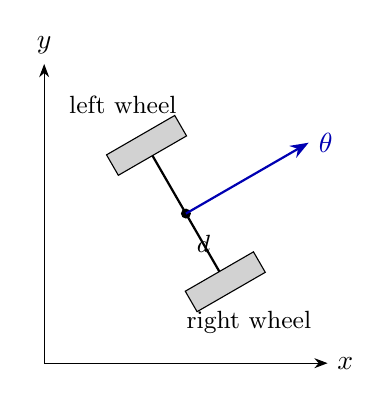
\begin{tikzpicture}[>=Stealth]
\coordinate (M) at (0,0);
\draw[->] (-1.8,-1.9)--(1.8,-1.9) node[right]{$x$};
\draw[->] (-1.8,-1.9)--(-1.8,1.9) node[above]{$y$};
\begin{scope}[rotate=30]
  \draw[thick] (0,-1)--(0,1);
  \draw[fill=gray!35] (-0.5,0.85) rectangle (0.5,1.15);
  \draw[fill=gray!35] (-0.5,-1.15) rectangle (0.5,-0.85);
\end{scope}
\fill (M) circle(1.8pt);
\draw[->,thick,blue!70!black] (M)--++(30:1.8) node[right]{$\theta$};
\node[font=\small] at ($(M)+(120:1.6)$) {left wheel};
\node[font=\small] at ($(M)+(-60:1.6)$) {right wheel};
\node[font=\small] at ($(M)+(-60:0.45)$) {$d$};
\end{tikzpicture}
\caption{Differential drive seen from above; the reference point is the midpoint of the axle.}
\end{figure}

\begin{intuition}
Worked numbers: $r=0.1$ m, $d=0.4$ m, $\omega_R=10$ rad/s, $\omega_L=6$ rad/s. Then $v=0.1\cdot16/2=0.8$ m/s and $\omega=0.1\cdot4/0.4=1$ rad/s, a turn of radius $v/\omega=0.8$ m. Equal wheel speeds give $\omega=0$ (straight line); opposite speeds give $v=0$ (rotation in place, the first and third phase of the universal maneuver).
\end{intuition}

\subsection{Synchro-drive}\emph{(page 8)}

A synchro-drive has three (or more) wheels that are steered and driven in a synchronized way, so that all wheels always point in the same direction $\theta$. The notes state that the KM \emph{is} the unicycle one and that \emph{no input transformation is needed}:
\[
\begin{cases}\dot x=\cos\theta\,v\\ \dot y=\sin\theta\,v\\ \dot\theta=\omega ,\end{cases}
\]
with $v$ the common driving velocity and $\omega$ the common steering velocity.

\begin{figure}[h]
\centering
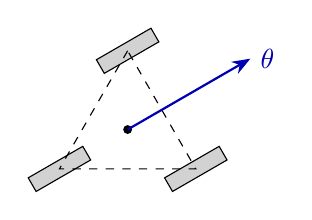
\begin{tikzpicture}[>=Stealth]
\coordinate (M) at (0,0);
\foreach \a in {90,210,330}{
  \begin{scope}[shift={(\a:1)},rotate=30]
    \draw[fill=gray!35] (-0.4,-0.1) rectangle (0.4,0.1);
  \end{scope}
}
\draw[dashed] (90:1)--(210:1)--(330:1)--cycle;
\fill (M) circle(1.6pt);
\draw[->,thick,blue!70!black] (M)--++(30:1.8) node[right]{$\theta$};
\end{tikzpicture}
\caption{Synchro-drive: three wheels steered together, all with orientation $\theta$.}
\end{figure}

\begin{intuition}
Because every wheel is always aligned with the others, the vehicle behaves as one big unicycle: the \emph{body orientation} that the model calls $\theta$ is the common steering angle. Unlike the differential drive, the physical inputs (driving and steering velocity of the synchronized wheels) already coincide with $(v,\omega)$, so the model works as is.
\end{intuition}

% =====================================================================
\section{Summary}
% =====================================================================

\begin{table}[h]
\centering\small
\renewcommand{\arraystretch}{1.25}
\begin{tabular}{@{}p{2.9cm}p{1.2cm}p{1.2cm}p{1.2cm}p{3.3cm}p{3.2cm}@{}}
\toprule
\textbf{System} & $\boldsymbol n$ & $\boldsymbol k$ & $\boldsymbol m$ & \textbf{Inputs $u$} & \textbf{Model}\\
\midrule
Unconstrained robot & $n$ & $0$ & $n$ & $u\in\R^n$ (fully actuated) & $\dq=u$ (canonical basis)\\
Unicycle & $3$ & $1$ & $2$ & $v$ (driving), $\omega$ (steering) & $\dq=g_1v+g_2\omega$\\
Differential drive & $3$ & $1$ & $2$ & $\omega_R,\omega_L\Rightarrow v=r\frac{\omega_R+\omega_L}2,\ \omega=r\frac{\omega_R-\omega_L}d$ & unicycle KM\\
Synchro-drive & $3$ & $1$ & $2$ & $v,\omega$ directly (no transformation) & unicycle KM\\
\bottomrule
\end{tabular}
\caption{Kinematic models covered. All are driftless and nonlinear in $q$; the three wheeled vehicles are controllable.}
\end{table}

\begin{figure}[h]
\centering
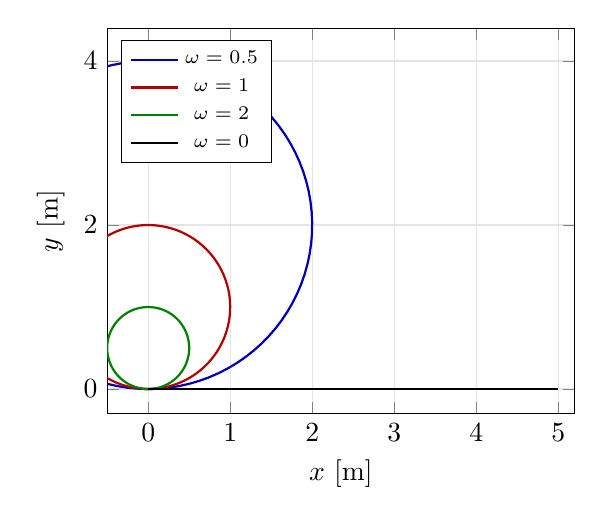
\begin{tikzpicture}
\begin{axis}[width=0.62\linewidth,axis equal image,xlabel={$x$ [m]},ylabel={$y$ [m]},
  xmin=-0.5,xmax=5.2,ymin=-0.3,ymax=4.4,legend pos=north west,legend style={font=\scriptsize},
  grid=both,grid style={gray!20}]
\addplot[blue!70!black,thick,domain=0:2*pi,samples=100] ({2*sin(deg(x))},{2*(1-cos(deg(x)))});
\addplot[red!70!black,thick,domain=0:2*pi,samples=100] ({1*sin(deg(x))},{1*(1-cos(deg(x)))});
\addplot[green!50!black,thick,domain=0:2*pi,samples=100] ({0.5*sin(deg(x))},{0.5*(1-cos(deg(x)))});
\addplot[black,thick] coordinates {(0,0)(5,0)};
\legend{$\omega=0.5$,$\omega=1$,$\omega=2$,$\omega=0$}
\end{axis}
\end{tikzpicture}
\caption{Unicycle with $v=1$ m/s, $q_i=(0,0,0)$ and constant $\omega$: circles of radius $v/\omega$ (straight line for $\omega=0$).}
\end{figure}

\subsection*{Key take-aways}
\begin{itemize}
\item Wheels impose Pfaffian constraints $A(q)\dq=0$; admissible velocities form $\N(A(q))$, of dimension $m=n-k$.
\item The kinematic model $\dq=G(q)u$ is a nonlinear, driftless system; $G$ is not unique, and bases are chosen for interpretability.
\item The unicycle ($n=3,k=1,m=2$) has $\dot x=v\cos\theta,\ \dot y=v\sin\theta,\ \dot\theta=\omega$; $v=r\omega_{\rm roll}$ is the driving velocity and $\omega$ the steering velocity.
\item Controllability of a KM is tied to nonholonomy of the constraints; the unicycle is controllable via the \emph{rotate--drive--rotate} maneuver.
\item Differential drive and synchro-drive share the unicycle KM (the former after the linear input change $v=r\frac{\omega_R+\omega_L}2$, $\omega=r\frac{\omega_R-\omega_L}d$).
\end{itemize}

\end{document}